% UCL Thesis LaTeX Template
%  (c) Ian Kirker, 2014
% 
% This is a template/skeleton for PhD/MPhil/MRes theses.
%
% It uses a rather split-up file structure because this tends to
%  work well for large, complex documents.
% We suggest using one file per chapter, but you may wish to use more
%  or fewer separate files than that.
% We've also separated out various bits of configuration into their
%  own files, to keep everything neat.
% Note that the \input command just streams in whatever file you give
%  it, while the \include command adds a page break, and does some
%  extra organisation to make compilation faster. Note that you can't
%  use \include inside an \include-d file.
% We suggest using \input for settings and configuration files that
%  you always want to use, and \include for each section of content.
% If you do that, it also means you can use the \includeonly statement
%  to only compile up the section you're currently interested in.
% You might also want to put figures into their own files to be \input.

% For more information on \input and \include, see:
%  http://tex.stackexchange.com/questions/246/when-should-i-use-input-vs-include


% Formatting rules for theses are here: 
%  http://www.ucl.ac.uk/current-students/research_degrees/thesis_formatting
% Binding and submitting guidelines are here:
%  http://www.ucl.ac.uk/current-students/research_degrees/thesis_binding_submission

% This package goes first and foremost, because it checks all 
%  your syntax for mistakes and some old-fashioned LaTeX commands.
% Note that normally you should load your documentclass before 
%  packages, because some packages change behaviour based on
%  your document settings.
% Also, for those confused by the RequirePackage here vs usepackage
%  elsewhere, usepackage cannot be used before the documentclass
%  command, while RequirePackage can. That's the only functional
%  difference as far as I'm aware.
\RequirePackage[l2tabu, orthodox]{nag}


% ------ Main document class specification ------
% The draft option here prevents images being inserted,
%  and adds chunky black bars to boxes that are exceeding 
%  the page width (to show that they are).
% The oneside option can optionally be replaced by twoside if
%  you intend to print double-sided. Note that this is
%  *specifically permitted* by the UCL thesis formatting
%  guidelines.
%
% Valid options in terms of type are:
%  phd
%  mres
%  mphil
%\documentclass[12pt,phd,draft,a4paper,oneside]{ucl_thesis}
\documentclass[10pt,mres,a4paper,oneside]{ucl_thesis}


% Package configuration:
%  LaTeX uses "packages" to add extra commands and features.
%  There are quite a few useful ones, so we've put them in a 
%   separate file.
% -------- Packages --------

% This package just gives you a quick way to dump in some sample text.
% You can remove it -- it's just here for the examples.
\usepackage{blindtext}

% This package means empty pages (pages with no text) won't get stuff
%  like chapter names at the top of the page. It's mostly cosmetic.
\usepackage{emptypage}

% The graphicx package adds the \includegraphics command,
%  which is your basic command for adding a picture.
\usepackage{graphicx}

% The float package improves LaTeX's handling of floats,
%  and also adds the option to *force* LaTeX to put the float
%  HERE, with the [H] option to the float environment.
\usepackage{float}

% The amsmath package enhances the various ways of including
%  maths, including adding the align environment for aligned
%  equations.
\usepackage{amsmath}

% Use these two packages together -- they define symbols
%  for e.g. units that you can use in both text and math mode.
\usepackage{gensymb}
\usepackage{textcomp}
% You may also want the units package for making little
%  fractions for unit specifications.
%\usepackage{units}


% The setspace package lets you use 1.5-sized or double line spacing.
\usepackage{setspace}
\setstretch{1.5}

% That just does body text -- if you want to expand *everything*,
%  including footnotes and tables, use this instead:
%\renewcommand{\baselinestretch}{1.5}


% PGFPlots is either a really clunky or really good way to add graphs
%  into your document, depending on your point of view.
% There's waaaaay too much information on using this to cover here,
%  so, you might want to start here:
%   http://pgfplots.sourceforge.net/
%  or here:
%   http://pgfplots.sourceforge.net/pgfplots.pdf
%\usepackage{pgfplots}
%\pgfplotsset{compat=1.3} % <- this fixed axis labels in the version I was using

% PGFPlotsTable can help you make tables a little more easily than
%  usual in LaTeX.
% If you're going to have to paste data in a lot, I'd suggest using it.
%  You might want to start with the manual, here:
%  http://pgfplots.sourceforge.net/pgfplotstable.pdf
%\usepackage{pgfplotstable}

% These settings are also recommended for using with pgfplotstable.
%\pgfplotstableset{
%	% these columns/<colname>/.style={<options>} things define a style
%	% which applies to <colname> only.
%	empty cells with={--}, % replace empty cells with '--'
%	every head row/.style={before row=\toprule,after row=\midrule},
%	every last row/.style={after row=\bottomrule}
%}


% The mhchem package provides chemistry formula typesetting commands
%  e.g. \ce{H2O}
%\usepackage[version=3]{mhchem}

% And the chemfig package gives a weird command for adding Lewis 
%  diagrams, for e.g. organic molecules
%\usepackage{chemfig}

% The linenumbers command from the lineno package adds line numbers
%  alongside your text that can be useful for discussing edits 
%  in drafts.
% Remove or comment out the command for proper versions.
%\usepackage[modulo]{lineno}
% \linenumbers 


% Alternatively, you can use the ifdraft package to let you add
%  commands that will only be used in draft versions
%\usepackage{ifdraft}

% For example, the following adds a watermark if the draft mode is on.
%\ifdraft{
%  \usepackage{draftwatermark}
%  \SetWatermarkText{\shortstack{\textsc{Draft Mode}\\ \strut \\ \strut \\ \strut}}
%  \SetWatermarkScale{0.5}
%  \SetWatermarkAngle{90}
%}


% The multirow package adds the option to make cells span 
%  rows in tables.
\usepackage{multirow}


% Subfig allows you to create figures within figures, to, for example,
%  make a single figure with 4 individually labeled and referenceable
%  sub-figures.
% It's quite fiddly to use, so check the documentation.
%\usepackage{subfig}

% The natbib package allows book-type citations commonly used in
%  longer works, and less commonly in science articles (IME).
% e.g. (Saucer et al., 1993) rather than [1]
% More details are here: http://merkel.zoneo.net/Latex/natbib.php
%\usepackage{natbib}

% The bibentry package (along with the \nobibliography* command)
%  allows putting full reference lines inline.
%  See: 
%   http://tex.stackexchange.com/questions/2905/how-can-i-list-references-from-bibtex-file-in-line-with-commentary
\usepackage{bibentry} 

% The isorot package allows you to put things sideways 
%  (or indeed, at any angle) on a page.
% This can be useful for wide graphs or other figures.
%\usepackage{isorot}

% The caption package adds more options for caption formatting.
% This set-up makes hanging labels, makes the caption text smaller
%  than the body text, and makes the label bold.
% Highly recommended.
\usepackage[format=hang,font=small,labelfont=bf]{caption}

% If you're getting into defining your own commands, you might want
%  to check out the etoolbox package -- it defines a few commands
%  that can make it easier to make commands robust.
\usepackage{etoolbox}


% Sets up links within your document, for e.g. contents page entries
%  and references, and also PDF metadata.
% You should edit this!
%%
%% This file uses the hyperref package to make your thesis have metadata embedded in the PDF, 
%%  and also adds links to be able to click on references and contents page entries to go to 
%%  the pages.
%%

% Some hacks are necessary to make bibentry and hyperref play nicely.
% See: http://tex.stackexchange.com/questions/65348/clash-between-bibentry-and-hyperref-with-bibstyle-elsart-harv
\usepackage{bibentry}
\makeatletter\let\saved@bibitem\@bibitem\makeatother
\usepackage[pdftex,hidelinks]{hyperref}
\makeatletter\let\@bibitem\saved@bibitem\makeatother
\makeatletter
\AtBeginDocument{
    \hypersetup{
        pdfsubject={Thesis Subject},
        pdfkeywords={Thesis Keywords},
        pdfauthor={Author},
        pdftitle={Title},
    }
}
\makeatother
    


% And then some settings in separate files.
% These settings are from:
%  http://mintaka.sdsu.edu/GF/bibliog/latex/floats.html

% They give LaTeX more options on where to put your figures, and may
%  mean that fewer of your figures end up at the tops of pages far
%  away from the thing they're related to.

% Alters some LaTeX defaults for better treatment of figures:
% See p.105 of "TeX Unbound" for suggested values.
% See pp. 199-200 of Lamport's "LaTeX" book for details.

%   General parameters, for ALL pages:
\renewcommand{\topfraction}{0.9}	% max fraction of floats at top
\renewcommand{\bottomfraction}{0.8}	% max fraction of floats at bottom

%   Parameters for TEXT pages (not float pages):
\setcounter{topnumber}{2}
\setcounter{bottomnumber}{2}
\setcounter{totalnumber}{4}     % 2 may work better
\setcounter{dbltopnumber}{2}    % for 2-column pages
\renewcommand{\dbltopfraction}{0.9}	% fit big float above 2-col. text
\renewcommand{\textfraction}{0.07}	% allow minimal text w. figs

%   Parameters for FLOAT pages (not text pages):
\renewcommand{\floatpagefraction}{0.7}	% require fuller float pages
% N.B.: floatpagefraction MUST be less than topfraction !!
\renewcommand{\dblfloatpagefraction}{0.7}	% require fuller float pages

% remember to use [htp] or [htpb] for placement,
% e.g. 
%  \begin{figure}[htp]
%   ...
%  \end{figure} % For things like figures and tables
% \bibliographystyle{unsrt}
\bibliographystyle{abbrvnat}
   % For bibliographies

\usepackage[english]{babel}
 
\usepackage{listings}

\usepackage{xcolor}
%\usepackage{amsmath}
\usepackage{amsfonts}
\usepackage{amssymb}
 
\definecolor{codegreen}{rgb}{0,0.6,0}
\definecolor{codegray}{rgb}{0.5,0.5,0.5}
\definecolor{codepurple}{rgb}{0.58,0,0.82}
\definecolor{backcolour}{rgb}{0.95,0.95,0.92}

\lstdefinestyle{pythonCode} {
    backgroundcolor=\color{backcolour},   
    commentstyle=\color{codegreen},
    keywordstyle=\color{magenta},
    numberstyle=\tiny\color{codegray},
    stringstyle=\color{codepurple},
    basicstyle=\ttfamily\footnotesize\bfseries,
    breakatwhitespace=false,         
    breaklines=true,                 
    captionpos=b,                    
    keepspaces=true,                 
    numbers=none,                    
    numbersep=4pt,                  
    showspaces=false,                
    showstringspaces=false,
    showtabs=false,                  
    tabsize=1
}
 \lstset{style=pythonCode}


 

% These control how many number sections your subsections will take
%    e.g. Section 2.3.1.5.6.3
%  and how many of those will get put into the contents pages.
\setcounter{secnumdepth}{3}
\setcounter{tocdepth}{3}


\usepackage{natbib}

% \usepackage{xcolor}

\begin{document}

\nobibliography*
% ^-- This is a dumb trick that works with the bibentry package to let
%  you put bibliography entries whereever you like.
% I used this to put references to papers a chapter's work was 
%  published in at the end of that chapter.
% For more information, see: http://stefaanlippens.net/bibentry

% If you haven't finished making your full BibTex file yet, you
%  might find this useful -- it'll just replace all your
%  citations with little superscript notes.
% Uncomment to use.
%\renewcommand{\cite}[1]{\emph{\textsuperscript{[#1]}}}

% At last, content! Remember filenames are case-sensitive and 
%  *must not* include spaces.
% I may change the way this is done in a future version, 
%  but given that some people needed it, if you need a different degree title 
%  (e.g. Master of Science, Master in Science, Master of Arts, etc)
%  uncomment the following 3 lines and set as appropriate (this *has* to be before \maketitle)
% \makeatletter
% \renewcommand {\@degree@string} {Master of Things}
% \makeatother

\title{Investigating and implementing neural network architectures for video classification}
\author{Olubunmi Aworanti}
\department{Department of Statistical Science}

\maketitle
\makedeclaration

\begin{abstract} % 300 word limit
  This paper investigates the design and building of different neural network architectures for video classification using tensorflow and the keras API. It begins by constructing a CNN Neural network architecture as described in \citep{KarpathyCVPR14}, using the keras API and tensorflow packages in python to build the required layer and models. these models where trained using the tensorflow UCF101 dataset. Finally it discusses minor adjustments made on model the performance and problems found with constructing and running these models.
\end{abstract}

\begin{acknowledgements}
Acknowledge all the things!
\end{acknowledgements}

\setcounter{tocdepth}{2} 
% Setting this higher means you get contents entries for
%  more minor section headers.

\tableofcontents
\listoffigures
\listoftables


\chapter{Introduction}
\label{chapterlabel1}
% Inline citation: \bibentry{example-citation}

\section{Aim}
The aim of this project is to understand how to implement neural network architectures and how they can be implemented given the software available today. The original goal was to create a machine vision tool for understanding emotion but in order to create such a tool one most first understand the basics of machine learning for image and video classification. The project is an exploratory one that follows my initial journey in understanding and implementing neural network architectures for video classification by first recreating architecture for action recognition in videos as presented in \bibentry{KarpathyCVPR14} using TensorFlow and the Keras API.

\section{Theory}
%needs more references%
\subsection{Neural networks}
To first begin we must understand what a neural network is, a neural network is a network of artificial neurons sometimes called a perceptron, a perceptron takes in an inputs $x_i$, and uses trainable weights $w_i$, a bias $b$ and a given activation function to predict the expected output $y_i$. Figure \ref{fig:neuron} provides an image representing a neuron. The activation functions commonly used include 

\begin{equation}
g(z) = \frac{1}{1+ exp(-z)}
 \qquad \text{Sigmoid function}
\end{equation}

\begin{equation}
g(z) = max(0,a)
 \qquad \text{Rectified Linear Unit(RELU) function}
\end{equation}

\begin{equation}
g(z) = \frac{exp(z)-exp(-z)}{exp(z) + exp(-z)}
 \qquad \text{Hyperbolic tangent function}
\end{equation}

\begin{figure}
  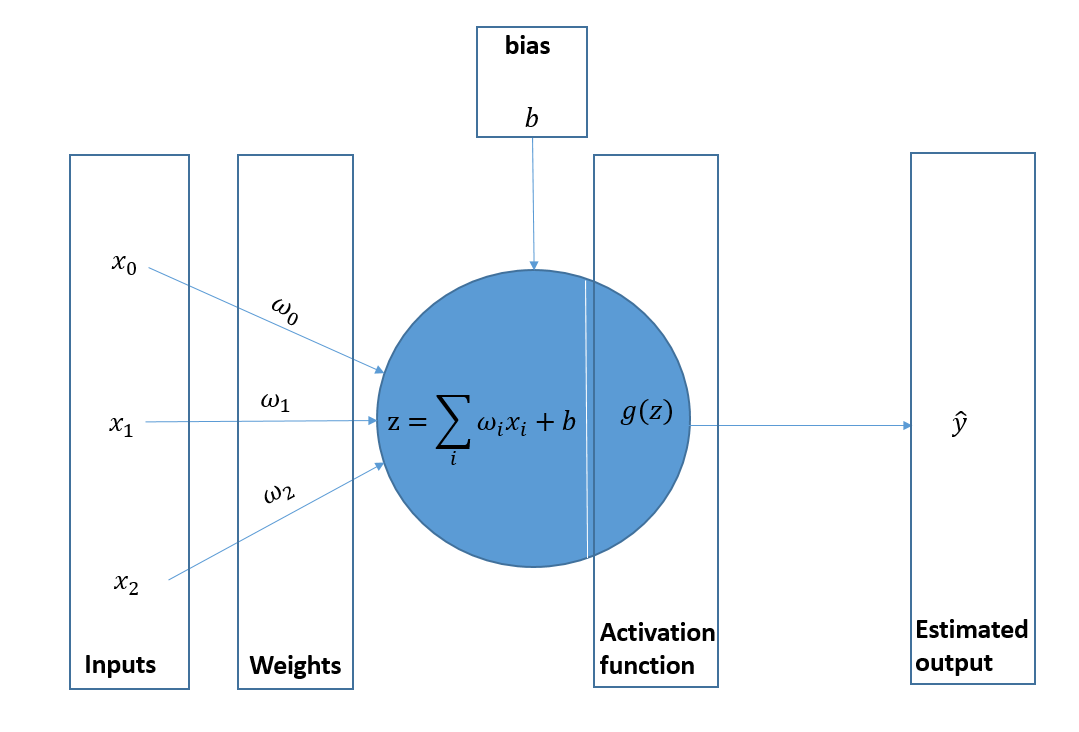
\includegraphics[width=\linewidth, scale=0.2]{neuron.PNG}
  \caption{Neural Network structure}
  \label{fig:neuron}
\end{figure}

To get accurate estimation of the output we have to decide on the weights and bias that would achieve this. One popular algorithm used for this is gradient decent. The gradient decent algorithm works as seen below. 
\begin{enumerate}
 \item  We begin by randomly initialize the weights and the bias
  \item then by what is called Forward propagation compute $z$ as seen in figure \ref{fig:neuron} then expected output given by the activation function. The formular $z$ can also be wriiten as $WX +b$ where  $W$ and $X$ are the matrix representation of the input and weights.
  \item Using a loss function, $\mathcal{L}(\hat{y},y)$ that compares the expected output and the estimated output, we can calculate the loss
  \item Our aim is to minimize this loss as much as possible so we do this by first calculating the partial derivative of the loss function with respect to the weight, $\frac{\partial \mathcal{L}(\hat{y},y)}{\partial W}$ and the bias, $\frac{\partial \mathcal{L}(\hat{y},y)}{\partial b}$
    \item Then using we can update the weight and bias using the below, where $\alpha$ is the learning rate.
\[W = W - \alpha \frac{\partial \mathcal{L}(\hat{y},y)}{\partial W}\]
\[b = b - \alpha \frac{\partial \mathcal{L}(\hat{y},y)}{\partial b}\]
\item We can then repeat step 2 to 5 till difference of current values and the updated values are at a expected threshold.
\end{enumerate}

We can stack these neurons together to from a neural network as seen in Figure \ref{fig:neuralnetwork}, which shows a 2 layer networks with one hidden layer with three neurons. The output of the activation function of the hidden layer servers as an input to the output layer. Usually the more complex the problem the deeper the network.
% maybe find  a diagram of the functions
In terms of activation functions, the RELU function is usually the activation function of choice for hidden layers. This is because there is less of an effect of the slope of the function as it goes to zero which allows for faster learning. The sigmoid function on the other hand is usually used in the output layer for binary classification.

\begin{figure}
  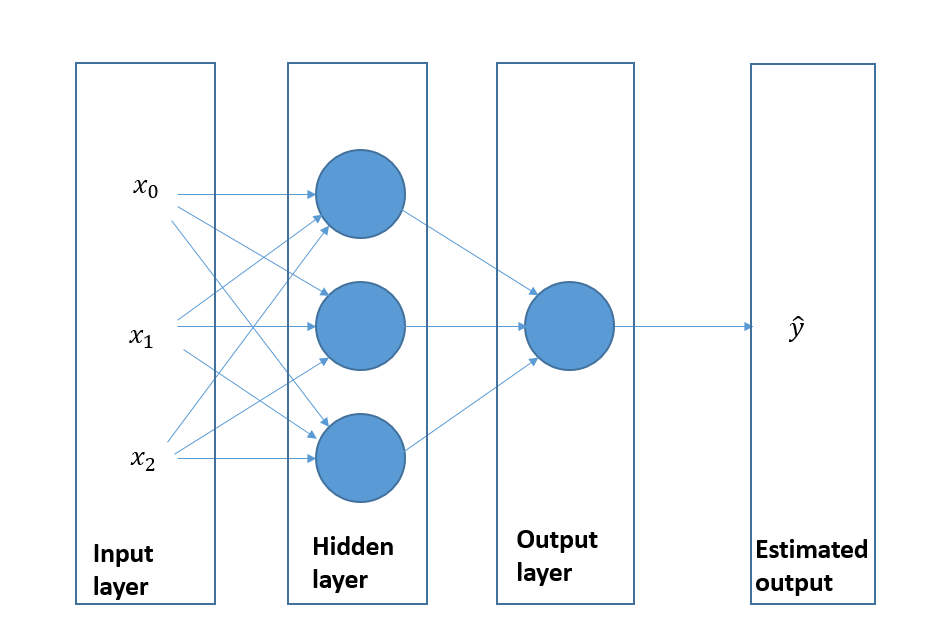
\includegraphics[width=\linewidth, scale=0.2]{multi-layer-network.PNG}
  \caption{Neural Network structure}
  \label{fig:neuralnetwork}
\end{figure}

\subsection{Convolutional Neural networks}
% also explain stride and give the formula for the parameters and where the features come in
Convolutional neural network, which will be the main network of focus in this project is simply a neural network mainly for inputs with a grid structure such as time series data and particularly images. These networks uses a convolution operation in place of a matrix multiple in atleast one of its layers as defined in \citep{Goodfellow-et-al-2016}. The convolution operation is typically represented with an asterisk:s  and seen below representing. 
\[ s(t) = (x * w)(t) \] 
which can be represented as the below, where $x$ is the input and $w$ is the kernal and the output is usually refered to as the feature map.
\[ s(t) = \int x(a) w(t - a)da \] 
In terms for matrices can be written as the below where $I$ for example is a two dimensional image and $K$ is the two dimensional kernel
\[S(i, j) = (I*K)(i, j) = \sum_m \sum_nI(m, n)K(i- m, j- n). \]
Convolutional networks also include a pooling layer which is a applys a function that replaces an input a with a summary statistic of the nearby input.

% \subsection{Optimization}



\section{Context}
    In past few years, with the increase in large labelled datasets such as the Imagenet dataset as discussed in \citep{JiaDeng2009IAlh}, which is an image dataset organized according to the WordNet hierarchy. In this hierachy, a wordnet is a meaningful concept which could also be described by multiple words or word phrases which are called a "synset". In the Imagnet dataset, WordNet contains more than 100,000 synsets, where nouns are the majority of about 80,000 plus. ImageNet aims to provide an average of 1000 images per each synset with the goal of offering tens of millions of images per WordNet. For video data of recent exist the YouTube-8M dataste as dicusssed in \citep{45619}, which a largest multi-label video classification dataset, composed of about 8 million videos for Youtube annotated with a vocabulary of 4803 visual entities. One intresting fact about the Youtube-SM dataset is that a Deep CNN pre-trained on ImageNet was also used to extract the hidden representation immediately prior to the classification layer showing how the available of large datassets can lead to progress in others. Not only have these datasets lead to growth with other datasets but most importantly they have also lead to a rise of various machine learning algorithms used to solve a diverse set of problems. Not only has the increase in datasets helped with this growth but also the increase in the available frames works and libraries used to create these various algorithms. some of these frameworks and libraries used for machine learning include scikitlearn which is a python programming language based library with a long range of user friendly API's for creating machine learning algorithms. \citep{DBLPjournalscorrBuitinckLBPMGNPGGLVJHV13} details the use of scikitlearn and its elegant APIs which has lead to a growth in implementation of models in the machine learning space. In the deep learning space, surveys such as \citep{Nguyen2019} have been taken on the available libraries and frameworks for deep learning with large datasets and the hardware requirements some of these frames works propose.\citep{Wang2019}, is another survey that details the more commonly used deep learning frame works developed by large software houses such as Google, Facebook, and Microsoft, and those developed by the open source community such as Caffe, Caffe2, Tensorflow, MXNet, CNTK, Torch, PyTorch,  MatconvNet, Matlab deep learning and Deep learning tool box, Deeplearning4j to name a few.
    For the purpose of this paper we will be looking at using Tensorflow and keras libraries and APIs with python as the programming language for building and using popular models. 
    Where Tensorflow is a free and open-source software library developed by Google and released in November 2015 for dataflow and differentiable programming as described in \citep{8578572} and keras as discussed in \citep{Lux:2019:OSC:3310195.3310202} is a high-level elegant neural networks API that provides tools for easy constructions of models. It also provides access to popular pre-trained models and it is capable of running on top of frameworks like TensorFlow, CNTK, or Theano. 
    This paper will be looking to experiment with how to implement neural network architectures for video classification particularly looking into deep convolutional neural networks which have been applied to a large pool of visual tasks since the late 1980s as discussed in \citep{doi:10.1162neco_a_00990}.
        % maybe add here more on video classification and temporal issues
    % Although primary used for image classification this paper will also be looking at the
    
        \section{Related Work}

% talk abour related work here on other models for video classification double check the pedistrain dection paper% 
There is vast range of problems in which convolutional neural network(CNNs) architectures are used, some of which are in the image classification space which include problems such as object detection for example in pedestrian detection \citep{TomeD2016DCNN} systems, to speech  recognition problems and also facial and body recognition systems which are items in the human emotion recognition and human interaction space \cite{knyazev2017convolutional} .They have also been used in natural language processing for example with modelling sentences as explained in \cite{Kalchbrenner_2014}. 
Most importantly, CNNs have also been used for video classification for example by using the codec as a spatio-temporal Activity Sensor on videos as described in \citep{ChadhaA2017VCWC}. Apart from convolutional neural networks there are other machine learning methods used for example bag of words models \citep{10.1007978-3-642-28493-9_34}, this can be based on using local visual descriptors, most common of these are histogram of oriented gradients (HOG), histogram of optical flow (HOF) and motion boundary histograms (MBH) descriptors which are very powerful for classification but also computationally expensive as described in \citep{Uijlings2015}. Other methods use recurrent neural networks(RNNs) which is also used in the natural language processing space and in general for sequence data. Since videos are essentially sequence data, RNNs can be used in theory however because RNNs are difficult to train on high-dimensional inputs due to the large input-to-hidden weight matrix there has been some difficulty using them, however there is additional research in the space that has lead to competitive results such as that described in \citep{yang2017tensortrain} which factorizes the input-to-hidden weight matrix using Tensor-Train decomposition to help with efficiency of training these models.
% reference need for von Neumann bottleneck and https://cloud.google.com/blog/products/ai-machine-learning/what-makes-tpus-fine-tuned-for-deep-learning%
Also when running these models apart from architecture one has to also consider processing hardware as evaluated in \citep{wang2019benchmarking} as this has an effect performance. Devices range (Central processing units) CPUs, which reads each instruction from the software hence has to store all calculaculations internally on memory. This memory access becomes the downside of CPU architecture called the von Neumann bottleneck because each CPU's Arithmetic Logic Units (ALU) executes calculation one by one, accessing the memory every time, limiting the total throughput and consuming significant energy. Another is the GPU(Graphical processing units which uses thousands of ALUs(about 2,500–5,000) in a processor of ALUs which means it can then execute thousands of multiplications and additions simultaneously. However it still suffers from the von Neumann bottleneck because For every  calculation in the thousands of ALUs, GPU it still needs to access shared memory to read and store intermediate calculation results. The most recent device of late is the Google designed, TPU (Tensor Processing Unit), which is designed as a matrix processor specialized for neural network work loads and is not as affected by the von Neumann bottleneck because its' primary task is matrix processing hence it consist of thousands of multipliers and adders connected to each other directly to form a large physical matrix called the systolic array architecture. Hence calculations naturally flow through the architecture reducing memory access during calculation and as a result it has a high computational throughput on neural network calculations with much less power consumption and smaller footprint.
%   todo add how easy it is to implement to bring it all together
  
%   such as there is a range of models typically used such as -----, videos can also be looked and complication of images in frames which simple convolutional networks can be use to classify together with methods used to take into account the temporal features. 
  
%   talk about vido clasification
    % This models have produced great results when it comes to image classification as discussed further in papers such as \citep{MISHKIN201711}. The use of convolutional neural networks doesn't stop in the computer vision field with image classification and video classification but also extends to tas well as physiological data, speech to name a few.
    
% why tensor flow this is a good paper \citep{schrimpf2016i}

    % When looking to build most reasches beging by either devloping there own neural network and looking at the archetures of other. one of the issue faces is the the same computational pwoer and hypter paraametres found.



\chapter{Theory}
\label{theory}
%needs more references%
\section{Neural networks}
\label{theory}
To first begin, building these convolutional neural networks,  we must understand what a neural network is.
A neural network is a network of artificial neurons.
These neurons are sometimes referred to as perceptrons.
A perceptron takes in an input $x_i$ and uses trainable weights $w_i$, a bias $b$ and a given activation function to predict the expected output $y_i$.
Figure \ref{fig:neuron} provides an image representing a neuron. The activation functions commonly used include 

\begin{equation}
g(z) = \frac{1}{1+ exp(-z)}
 \qquad \text{Sigmoid function}
\end{equation}

\begin{equation}
g(z) = max(0,z)
 \qquad \text{Rectified Linear Unit(RELU) function}
\end{equation}

\begin{equation}
g(z) = \frac{exp(z)-exp(-z)}{exp(z) + exp(-z)}
 \qquad \text{Hyperbolic tangent function(Tanh)}
\end{equation}

\begin{equation}
g(\mathbf{z}) = \frac{exp(z_i)}{\sum_{j=1}^{K}exp(z_j)} \textrm{ for } i = 1,...,K \textrm{ and } \mathbf{z} = \{ z_1,....,z_K \} \in \mathbb{R}^K
 \qquad \text{Softmax}
\end{equation}

\begin{figure}
\centering
  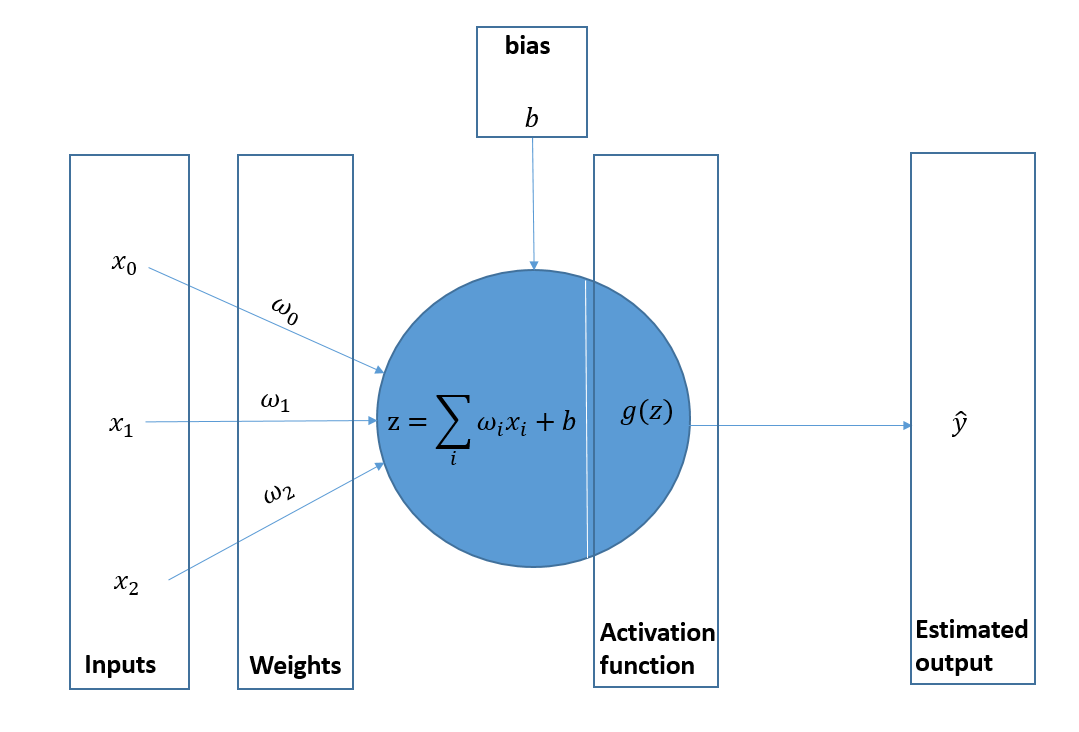
\includegraphics[width=75mm,scale=0.75]{neuron.PNG}
  \caption{Neuron}
  \label{fig:neuron}
\end{figure}

%todo stats around these activation functions.
Figure \ref{fig:activations} shows the plot of the sigmoid, RELU and Tanh activation functions. The sigmoid function gives an output between [0,1]. The RELU function also gives an output between [0,1], but it gives an output of 0 for inputs less than 0.  While the Tanh function gives an output between [-1,1].  The sigmoid function is usually used for binary classification while the softmax activation function is usually used for multi-class classification.  This is because the softmax function calculates the probabilities distribution of the output class $z_i$  over the different possible output classes.
\begin{figure}
\centering
  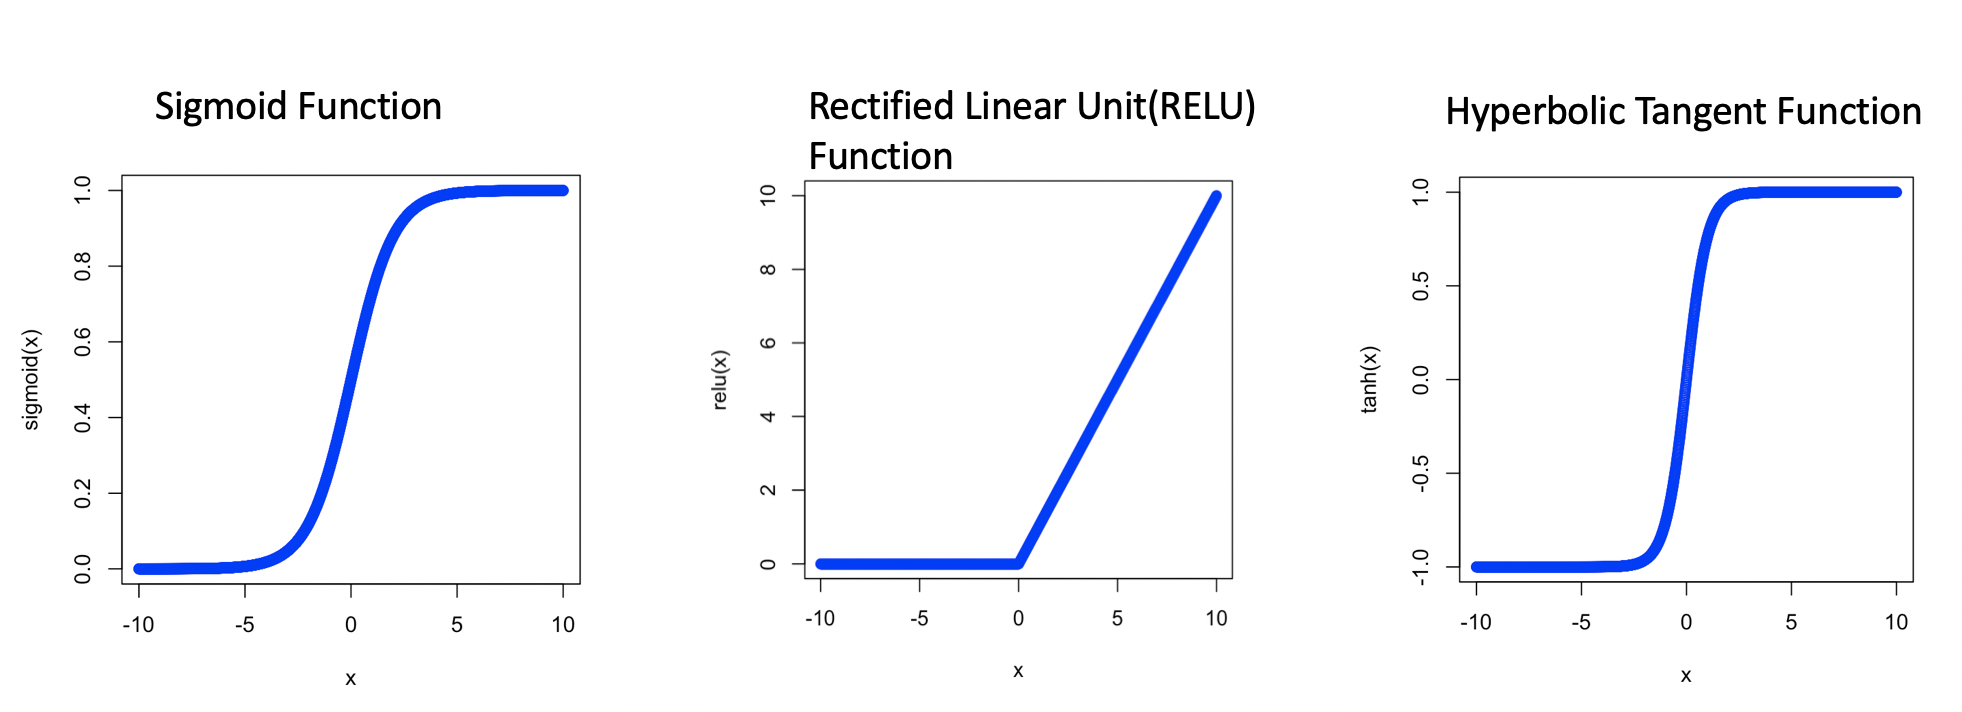
\includegraphics[width=\linewidth, scale=1]{activations.png}
  \caption{Plot of sigmoid, RELU and Tan-h activation functions}
  \label{fig:activations}
\end{figure}
%todo crosscheck  gradient decent function and show more of the chain rule %
To get an accurate estimation of the output, the weights and bias that would achieve this, have to be estimated. One popular algorithm used for this is gradient descent. The gradient descent algorithm aims to minimize this loss. Its steps can be seen below. 
\begin{enumerate}
 \item  Randomly initialize the weights and the bias
 \item Forward propagation, compute $z$ as seen in figure \ref{fig:neuron}, then use $z$  to calculate the expected output using the activation function. 
  \item Using a chosen loss function, $\mathcal{L}(\hat{y},y)$ that compares the expected output and the estimated output, we can calculate the loss.
  \item Calculate the partial derivative of the loss function with respect to the weight, $\frac{\partial \mathcal{L}(\hat{y},y)}{\partial w}$ and the bias, $\frac{\partial \mathcal{L}(\hat{y},y)}{\partial b}$. These partial derivative are arrived at via  backpropagation, which involves using the chain rule. With backpropagation, for example $\frac{\partial \mathcal{L}(\hat{y},y)}{\partial w } = x\frac{\partial \mathcal{L}(\hat{y},y)}{\partial \hat{y} } \frac{\partial \hat{y}}{\partial z }  $  and $\frac{\partial \mathcal{L}(\hat{y},y)}{\partial z} = \frac{\partial \mathcal{L}(\hat{y},y)}{\partial \hat{y} } \frac{\partial \hat{y}}{\partial z }  $.
    \item Update the weight and bias using the below, where $\alpha$ is the learning rate.
\[W = W - \alpha \frac{\partial \mathcal{L}(\hat{y},y)}{\partial W}\]
\[b = b - \alpha \frac{\partial \mathcal{L}(\hat{y},y)}{\partial b}\]
\item Repeat step 2 to 5 till difference of current values and the updated values are at a expected threshold.
\end{enumerate}

Note that the formula $z$ can also be written as $W^TX +b$. Where  $W$  and $X$ are the matrix representation of the input and weights of size, $n \times m $  respectively.  Moreover, $b$ is a $n  \times n$ size vector of the biases.
%more of an explanation
There is a range of loss functions used that are usually linked to an activation function. One loss for binary classification is the log loss which can be written as $ -(y \log{(\hat{y})} + (1-y)\log(1-\hat{y} ))$ when the are two classes and the discrete $ - \sum_{j=1}^{K} y\log{\hat{y}} $ for multi-classification. It is also referred to as cross-entropy loss. Sparse cross-entropy loss is an extension of cross-entropy loss, where the outputs are mutually exclusive.  Meaning each input can only belong to one output class and represent using one-hot embeddings.

When neurons are stacked together, they form a neural network as seen in Figure \ref{fig:neuralnetwork}. This shows a 2 layer network with one hidden layer with three neurons. The output of the activation function of the hidden layer servers as an input to the output layer. Usually, the more complex the problem, the deeper the network.
% maybe find  a diagram of the functionsWhen using gradient decent ,  The RELU function is usually the activation function of choice for hidden layers. This is because the RELE function has  less of an effect when the slope function goes to zero, as seen in \ref{activations}, which allows for faster learning. 


\begin{figure}
\centering
  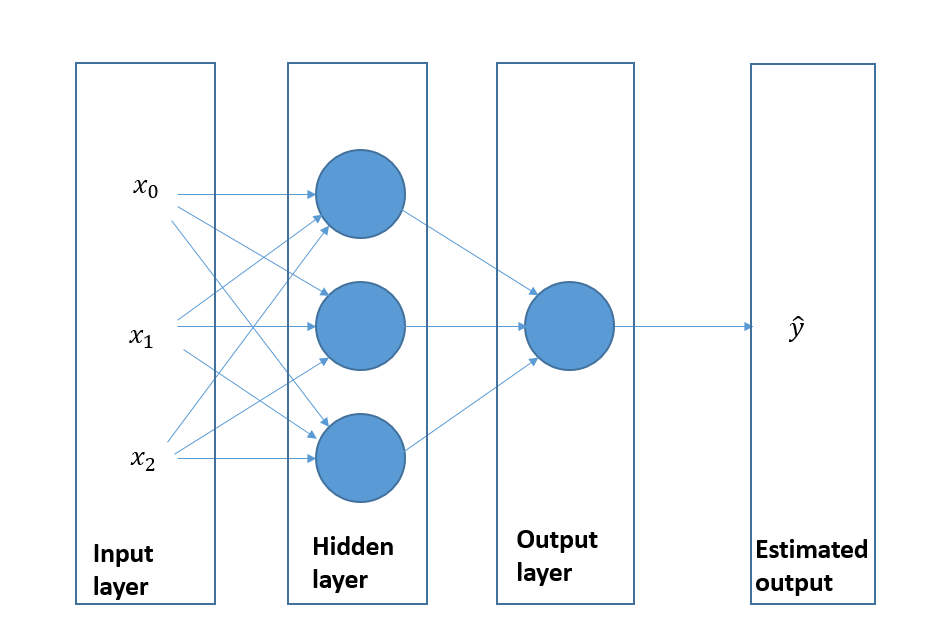
\includegraphics[width=75mm,scale=0.75]{multi-layer-network.PNG}
  \caption{Neural Network structure}
  \label{fig:neuralnetwork}
\end{figure}

\section{Optimization}
% todo find papers for all these regularzation%
The performance of a neural network can be affected by a range of items. This includes the learning rate, the number iterations before the gradient descent algorithm converges, the number of hidden layers, the number of hidden units in each layer and the activation function to name a few.  
These items are referred to as hyperparameters. 

%maybe add dev set%
When evaluating the performance of a neural network, it is best to separate the input data into a training and test set. A standard split of training to test set is about 70%, 30% for a dataset with a size of up to 10000.  The training dataset is used to train the model and arrive at the best possible weights and bias. The test dataset is then used to evaluate the model's performance based on the final parameters, i.e. is the weights and biases. The metric of performance is usually the accuracy which is the percentage of the model's output which was predicted correctly.

When training, it is best to avoid overfitting, i.e. when there is high variance, and the model does better on the training set than on the test set. Underfitting also needs to be avoided. 
Underfitting is when there is a high bias, and the model does not perform well on the training set. 
The usual process is to first combat underfitting by building a model that fits the training data. This can be done by increasing the number of hidden layers or nodes in a hidden layer hence increasing the parameters that fit the data.  Once the train data has been fitted, and the parameters decided, the model is then validated against the test set. If overfitting occurs, the following regularization techniques can be applied to reduce the parameters as listed below:
\begin{itemize}
    \item Dropout - This involves setting a probability at which to drop a percentage of nodes in order to reduce the number of parameters 
    \item Early Stopping -  this involves stopping the training at an early stage. By stopping the training at an early stage, it reduces the size of the parameters learned. 
    \item Data Augmentation - One cause of overfitting is the lack of varied data. Data augmentation is mainly used in the image classification space to reduce the issue of varied data. It involves applying various augmentation techniques such as horizontal flipping, random cropping, to produce a more varied training set. 
\end{itemize}

%Add equations for this%
When dealing with a large dataset, gradient descent can take a long time to process. As it completes one update step over the whole dataset. Various optimization techniques can be used to reduce this time. Some of these include Stochastic gradient descent which works by first shuffling the data, then updating the parameters for each training set. Another is mini batch gradient descent which takes a subset of the data called batches on which the parameters are updated. The batches sizes are usually in factors of 32 because it allows for easier computing. Usually when implementing models, a step is refers to one iteration in which one batch is processed and an epoch  referes to when the whole dataset i.e. all the batches for the dataset has been processed. Other optimizations are RMS prop and Adam optimization, which help with the smoothness of the gradient descent using various hyperparameters and theories such as exponentially weighted averages.
 
Another essential item is normalization; usually, when the input to a neuron is normalized, it tends to train better. In deeper neural networks, there have also been benefits found with normalizing the linear input $z$ to each activation function at every layer. Some of these normalization techniques include local response normalization and batch normalization.



\section{Convolutional Neural networks}
%maybe talk about the flipping%
% also explain stride and give the formula for the parameters and where the features come in
A convolutional neural network is simply a neural network mainly for inputs with a grid structure such as time-series data and particularly images. The network uses a convolution operation in place of matrix multiplication in at least one of its layers as defined in \citep{Goodfellow-et-al-2016}. The convolution operation is typically represented with an asterisk:s  and seen below representing. 
\[ s(t) = (x * w)(t) \] 
where $x$ is the input, and $w$ is the kernel, and the output is usually referred to as the feature map.
\[ s(t) = \int x(a) w(t - a)da \] 
In terms of matrices, it can also be written as the below where $I$ for example is a two-dimensional image and $K$ is the two-dimensional kernel
\[S(i, j) = (I*K)(i, j) = \sum_m \sum_nI(m, n)K(i- m, j- n). \]
Convolutional networks also include a pooling layer which applies a function that replaces an input with a summary statistic of the nearby inputs, sometimes reducing the input matrix size.

By applying specific kernels to input, in the case of image recognition, a layer can learn specific features of the image such as edge detection for example. When applying a  kernel to an input, the output is usually reduced as seen in figure \ref{fig:convolution}. With the reduced output in order to prevent a shrinking output as we go deeper into a network and to hold more information on the image, padding can be applied. Padding involves adding a border containing $p$  pixels to the image.  This leads to an increase in the output size as a kernel is applied. Another essential term, in convolutional neural networks, is stride. Stride involves taking  $s$ steps for the element-wise multiplication with the kernel, rather than 1 step. When a kernel of $f \times f$  is applied to an image of  $n \times n $  with a stride of $s$ and a padding  $p$,  the resulting output size is given by the equation 

    
\[ \left[ \frac{n + 2p -f }{s} +1 \right]   \times  \left[ \frac{n + 2p -f }{s} +1 \right]
\]

Convolutional neural networks can also take in a volume input by simply be extending the kernels over the dimensions of the input.  


\begin{figure}
\centering
  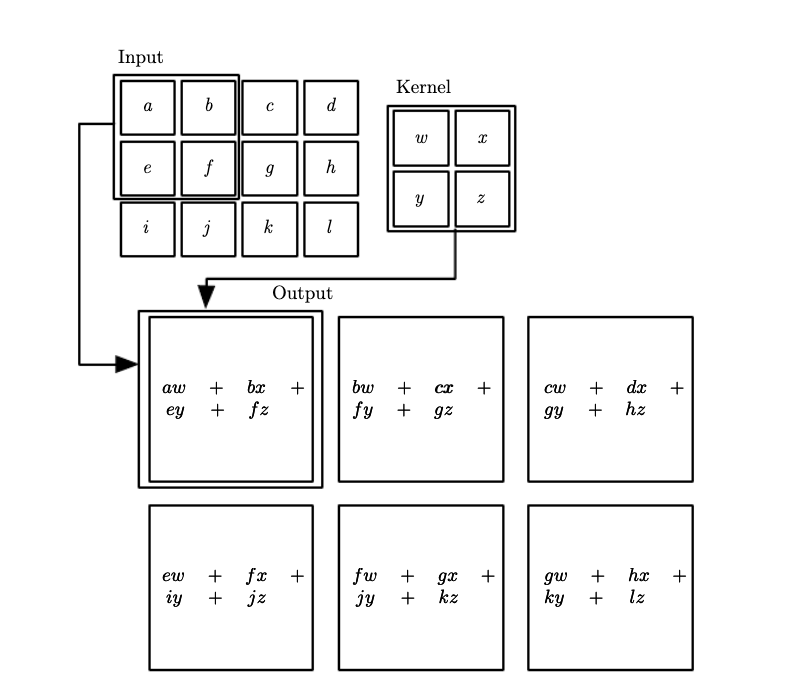
\includegraphics[width=75mm,scale=0.75]{convolution.png}
  \caption{Convolution operation without flippings sourced from \citep{Goodfellow-et-al-2016}}
  \label{fig:convolution}
\end{figure}







\chapter{Setup}
\label{chapterlabel2}
% \section{Overview}
%As mentioned previously,  this project looks to implement convolutional networks for video classification, particularly looking at action labelled data.
% explain convultional netweorks with pooling layer

% with the future aim of exploring with emotion classification using image and video data. Something that has been explored in papers such as \cite{SUN201836}
% explain f what a convutional neural network is here, talk about Alexnet
% In order to get familiar with building neural networks, the first task involved  then understanding the structure and looking atthe performance of pretrained models CNN models readily available.



\section{Environment and Software}
% todo explain the clusters better
%what is pip
Since the project required TensorFlow and the Keras API with python programming language, python 3.6 was used as it is the newer and more compatible python version from the legacy soon to be deprecated python 2.7.
The initial coding environment set up was done using Anaconda which is  an open-source distribution for python and python libraries which are typically used for scientific computing. Anaconda also provides distribution of other statistical tools such as R-studio which is used for the R programming language.
Another benefit of Anaconda is that it allows for multiple python environments and easy download of libraries. It has a very friendly user graphical interface as well as a command-line interface.
%todo pip and reference
Pip which is the python specific library management tool, was also used to download some TensorFlow libraries which were not available in Anaconda.

TensorFlow comes in two distribution the first being the Graphics processing unit (GPU) enabled distribution with uses the GPU first by default to speed up specific processes before it uses the (Central processing unit ) CPU.
The second distribution, which is also the default distribution runs on the CPU only.
The project initially began on a laptop with no GPU capacity. Hence the TensorFlow default package was installed.

The impressive quality of TensorFlow, is its use of a dataflow graph. In the TensorFlow dataflow graph, the nodes represent units of computation, and the edges represent the input data or the output data of the computation. This dataflow graph allows for benefits such as the use of parallel computing for model training ad running, distributed execution through the use of explicit edges which allows for partitioning across multiple devices. The dataflow graph also improves compilation and generates faster code by allowing TensorFlow's XLA compiler to use dataflow graph information. The dataflow graph is also language-independent, allowing for portability between language.
TensorFlow comes with a keras API within its libraries, this version of Keras supports the use of the dataflow graph unlike the readily available Keras library.  As TensorFlow provides the Keras API,  there was no need to download keras separately.
The project also initially began in a jupyter notebook environment which is an open-sourced web-based interactive development environment used for a multitude of scientific research. An Empirical Study on Jupyter notebook as a tool for scientific research has also been taken as seen in \citep{Randles_2017}. While on jupyter notebook, TensorFlow was running in eager mode.  Eager mode is a programming environment provided by TensorFlow which evaluates operations from the dataflow graph immediately. It does this by not building computational graphs, hence allowing concrete values to be returned instead of constructing a graph to run later, making debugging easier in such an interactive environment like jupyter notebook.
Once familiar with the working of the Tensorflow environment, The models were then transferred into python scripts.

% Rather building models from scracth the TensorFlow package and keras  packages where used to construct the models and access the pre-trained models.

\section{Datasets}
TensorFlow also provides readily available pre-processed data sets for easy use. These datasets are available using the TensorFlow dataset library. The TensorFlow dataset is a library that exposes publicly available datasets as numpy arrays, TensorFlow dataset object or tensors. The datasets range from images to audio to text datasets. Some popular datasets include MNIST database of handwritten digits \citep{6296535}. 
This project used the UCF101 dataset provided by TensorFlow dataset library. The UCF101 dataset is an action recognition dataset of realistic action videos, collected from YouTube, having 101 action categories \cite{soomro2012ucf101}. It contains about 13320 videos for the 101 action categories. The videos in the 101 action categories are grouped into 25 groups, where each group can consist of 4-7 videos of an action. The videos from the same group may share some common features, such as similar background, similar viewpoint, etc.
The action categories can be divided into five types which include Human-Object Interaction, Body-Motion Only, Human-Human Interaction , Playing Musical Instruments and Sports.
Tensorflow also provides a train test split of the data where the number of training examples is 9537, and the number of test examples is 3783.
It also provides the functionality to take a custom spilt of the data and reduce the number of videos used for training. Each clip contains multiple frames of 256x256x3. The frames were taken at a  rate of 25 fps. The clips range in length from about 1.06 seconds to  71.04 seconds.
%todo crosscheck how youtube-8m download works%
This UCF101 dataset is also used in \citep{KarpathyCVPR14} to train models based off pre-trained models trained with the larger data set of sports-1M.
The  sports-1M dataset, which consists of over one million YouTube videos belonging to about 487 classes of sports which was used \citep{KarpathyCVPR14}. Could not be used because although it is readily available on youtube with most of the links supplied in it's GitHub repository.  This is because downloading a dataset of that magnitude proposes a challenge with the memory needed to store the dataset — also the time required in downloading this large dataset. Such a large dataset can also lead to extremely long training time. There is also the challenge of copyright as no clear instructions on copyright was set for all the applicable videos from Youtube. Hence because of this and the time constraints with the project, the smaller UCF101 dataset was used to recreate the models. It is also important to note that the sports-1M is also available as part Youtube-8M dataset. And although there is an API available to download videos from the Youtube-8M as TensorFlow Record file, the sports-1M dataset cannot be easily specified for download from the Youtube-8M as it does not allow for access to specific videos. Which would have been an excellent addition because the sport-1M dataset GitHub page provides the list of videos included in the sport-1M dataset split into training and test datasets.

% might be worth summaring the dataset used in karpathy's paper

\section{Computation}
Most of the models had a long-running time when ran in the jupyter notebook environment, So it needed to be run over a long period of time with a capable computer infrastructure.  Then UCL cluster infrastructure was then used for running the models. The scripts were initially run in the cluster log in the terminal. Then they were running for a short time, in the interactive session, which allows the setup of the required memory and processing power needed to run. This was used to gauge the right setup by comparing the speed per each epoch and step for different configurations.  Once decided on the setup, such as the RAM required and the number of GPUs required. The clock time, which is how long the model will run for was decided. Then the batch jobs were set up to run the models from the python scripts.


\section{Architectures}

In \citep{KarpathyCVPR14} paper on Large-scale Video Classification with Convolutional Neural Networks \citep{KarpathyCVPR14}, it discusses various models and explores approaches for fusing information over temporal dimension through the convolutional network and compares their performance. Using the UCF101 dataset and TensorFlow, this project will also explore recreating these models and apply newer techniques for optimization. The models which will be implemented are listed below. The structures of these models can be also be seen in figure \ref{fig:k_models} taken from \citep{KarpathyCVPR14}
\begin{itemize}
    \item Single Frame: is loosely based on the Alexnet model \cite{NIPS2012_4824}, which was the winning model of the ImageNet challenge in 2012. Alexnet model takes in an input image of $224 \times 224 \times 3$, using the shorthand notation as described in \citep{KarpathyCVPR14}, the full architecture is $C(96, 11, 4)-N-P-C(256, 5, 1)-N-P-C(384, 3, 1)-C(384, 3, 1)-C(256, 3, 1)-P-F C(4096)-F C(4096)$, where $C(d, f, s)$, is a convolutional layer with d filters of spatial size $ f × f$, with a stride of $s$,  $FC(n)$ is a fully connected layer with n nodes, $N$ is local response normalization layer and P is the pooling layer. The single frame model from \cite{KarpathyCVPR14} follows the following architecture  $C(96, 11, 3)-N-P-C(256, 5, 1)-N-P-C(384, 3, 1)-C(384, 3, 1)-C(256, 3, 1)-P-F C(4096)-FC(4096)$ with the exception that it takes in an image of size $ 170 \times 170 \times 3$. The single frame also uses a max-pooling of a non-overlapping with size $2 \times 2$ rather than overlapping pooling of size $3x3$ and stride $2$ used in the Alexnet. This is an interesting difference that might have an effect on performance as the Alexnet paper suggest that generally, they observed during training that models with overlapping pooling found it slightly more difficult to overfit.
    \item Early Fusion - This combines information across an entire time window immediately on the pixel level hence making the input size that of $11 \times 11 \times 3 \times T$ pixels, where T was 10 which is also the number of frames covered. The change in input shape also required a change to the first convolutional layer to use a filter size of $10 \times 11 \times 11$.
    \item Late Fusion: This uses two single frame networks that have input frames that are about 15 frames apart. The single frame networks are combined at the fully connected layers.
    \item Slow Fusion: This is a mix of both late and early fusion. It slowly combing the temporal information over at each convolutional layer. The input is a set of 10 frames from a clip. The first convolution layer now consists of 4 parallel layers that each take in 4 frames out of the initial 10 frames, The second convolutional layer consist of two parallel layers that combine the two outputs from the first while the third layer combines the output from the second layer
\end{itemize}

\begin{figure}
    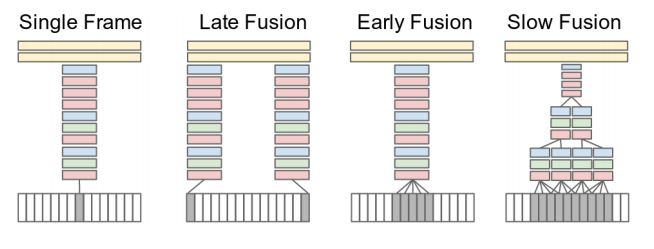
\includegraphics[width=\linewidth]{K_models.JPG}
    \caption{\citep{KarpathyCVPR14} Explored approaches for fusing information over temporal dimension through the network.  The Red, Green and Blue boxes indicate convolutional, normalization and pooling layers respectively}
    \label{fig:k_models}
\end{figure}

There is a wide range of a pre-trained convolution neural networks architectures particularly models for image classification trained on ImageNet dataset available via the Keras API.  A few of these where also explored as listed below.
\begin{itemize}
    \item VGG19: as described in \citep{simonyan2014deep}, is quite a standard convolutional neural network architecture that consists of a $3 \times3$  filters with a stride 2, followed by a $2\times2$ max-pool filter with a stride of 2.
    \item MobileNetV2: is a model created for mobile vision application a. MobileNetV2 as discussed in \cite{Sandler_2018} improves on its predecessor MobileNetV1 as discussed in \citep{howard2017mobilenets}.  MobileNetV1 uses a depthwise separable convolution as efficient building blocks while MobileNetV2 introduces a linear bottleneck between the layers and a shortcut connections between the bottlenecks.
    \item Inception: this convolutional neural network architecture as discussed in \citep{Szegedy_2016} is made up of inception blocks which evaluate multiple, multiple pooling layers of different dimensions then concatenate the results.
    \item ResNet: this architecture \citep{He_2016} is made up of residual blocks. These residual blocks are a set of two layers that rather than going through the standard path of going from one activation layer to the next, passes the linear equation output to the next layer activation function to arrive at the activation value for the next layer. This is believed to have the benefit of helping with vanishing and exploding gradients to improve performance as the neural network gets deeper.
\end{itemize}


\section{Assumptions}
Some assumptions were made on the implementation of the models such as the starting frame for the model inputs.  This was because it was not explicitly made clear in the text in \citep{KarpathyCVPR14}. Although one could argue that in figure \ref{fig:k_models}, the 7th frame from the start point of the model was used.  However, initially, all model implementation, the first frame was selected as the starting frame. For example, this means with the single frame implementation, the first frame of the clip was the input frame.  The seemed like a modest assumption because as discussed in \citep{soomro2012ucf101} which discussing the UCF101 dataset, the videos have a huge variation in length hence to avoid any issues such as selecting a frame in a position that does not exist.

In \citep{KarpathyCVPR14}, they talk about using downpour stochastic gradient descent to optimize the models across a computing cluster. They used about 10 to 50 replicas for each model; they further split every model across 4 to 32 partitions. They also use mini-batches of 32 examples, momentum of 0.9, weight decay of 0.0005 and a  learning rates of $1e^{-3}$, which was further reduced by hand whenever the validation error stops improving.  However, for this project, a more simplified optimization was used which was inspired from \citep{KarpathyCVPR14}. The optimization uses initially for all models was a stochastic gradient descent with mini-batches of 32 examples, momentum of 0.9, weight decay of 0.0005 and a static learning rates of $1e^{-3}$.

\citep{KarpathyCVPR14} also does not specify the loss function used; however, since there was a reasonably large number of categories for the UCF101 dataset sparse categorical cross-entropy seemed like the best option. This was also because unlike its counterpart categorical cross-entropy which is also used for multi-classification; sparse categorical cross-entropy requires a one-hot encoded. 

A standard accuracy performance metric was also used when  training and validating the model as none where specifically specified in \citep{KarpathyCVPR14}

%and the first frame with is extended for the other models such as the late fusion and slow fusion models%

\chapter{My Second Content Chapter}
\label{chapterlabel3}

\section{Coding}
% -	I’d suggest separating custom contributions to the code from set-up of the experiment. Currently, some things I’d expect in the latter chapter are here.
% -	Also, you don’t need to explicitly present all of your code. Better attach it, or provide a github link, and highlight only relevan parts if you need to.

     
The coding began by first importing the tensorflor and tensorflow dataset.

\begin{lstlisting}[language=Python, caption=Importing tensorflow libaries]
import tensorflow as tf
import tensorflow_datasets as tfds
\end{lstlisting}

Using the tensorflow dataset libary allowed for easy loading of the UCF101 dataset as seen below. The libary also provides a default recommeneded train and test dataset. It also provided an information object detailing the labal and dataset size for the train and test size. 
     
\begin{lstlisting}[language=Python, caption=Loading UCF101 dataset]
ucf101_dataset, ucf101_info = tfds.load(name="ucf101", with_info=True)
ucf101_train , ucf101_test = ucf101_dataset["train"], ucf101_dataset["test"]
\end{lstlisting}

% todo talk about batches and shuffling

Custom python helper methods where used for the formatting of the images in the frame from $256 \times 256 \times 3$ to $170 \times170 \times 3$ as suggested in \citep{KarpathyCVPR14}. Most layers needed to build the model where present in the keras API. Most models where implemented using the keras sequential model which is the simplest model to implement as it is a simply a linear stack of layers as seen below. The single frame layer for example was implemented as a keras sequential model by passing in a list of layers as seen in \ref{singleFrame} note that this can also be implemented by using the the keras API add method to add in layers. More complex architectures such as the slow fusion layer used the keras functional API which uses the fact that a layers is a callable instance that can be called on a tensor and then returns a tensor to build multi-output and multi-input models like the slow and late fusion model.

\begin{lstlisting}[language=Python, caption=Single Frame model implemetation, label=singleFrame]
model = tf.keras.models.Sequential([
    tf.keras.layers.Conv2D(96, (11,11), strides=3 , activation='relu', input_shape=(170, 170, 3)),

    l.MyLRNLayer(),
    tf.keras.layers.MaxPooling2D(2, 2),
    tf.keras.layers.Conv2D(256, (5,5), strides=1, activation='relu'),

    l.MyLRNLayer(),
    tf.keras.layers.MaxPooling2D(2, 2),
    tf.keras.layers.Conv2D(384, (3,3), strides=1, activation='relu'),

    tf.keras.layers.Conv2D(384, (3,3), strides=1, activation='relu'),
    tf.keras.layers.Conv2D(256, (3,3), strides=1, activation='relu'),

    tf.keras.layers.MaxPooling2D(2,2),
    tf.keras.layers.Flatten(),

    tf.keras.layers.Dense(4096, activation='relu'),
    tf.keras.layers.Dense(4096, activation='relu'),
    tf.keras.layers.Dense(101, activation='softmax')
])
\end{lstlisting}

%todo more on the difference between LRN and batch normalization%
Some custom layers where needed like the local response normalization layer as described in \citep{NIPS2012_4824}. This was because it was no longer available on the keras API. As the local response normalization is a non-trainable layer normalizes values in a feature map within a local making less adaptive. While its replacement batch normalization as discussed in \citep{ioffe2015batch} is a trainable normalization layer wich allows for a much higher learning rates and requires less care with initialization. Batch normalization in some cases is also said to eliminate the need for Dropout. 
Another benefit of the Keras API is how it allows for easy creation of a custom layers through inheritance from its keras layer class as seen in \ref{lrn}. Here since all the parameters of the LRN are fixed no training is required hence the layer is set to trainable false.
This implementation also utilizes the tensorflow nn API which holds a functions that can be applied to tensor. Fortunately it also offers a local response normalization layer function calculation which returns the normalized tensor hence this was wrapped in the keras layer object so it can be used in  keras sequential model to implement the models.

\begin{lstlisting}[language=Python, caption=Local response normalization layer implemetation, label=lrn]
class MyLRNLayer(tf.keras.layers.Layer):
    def __init__(self, depth_radius=5,bias=1,alpha=1,beta=0.5, **kwargs):
        #         self.output_dim = output_dim
        self.depth_radius = depth_radius
        self.bias = bias
        self.alpha = alpha
        self.beta = beta
        super(MyLRNLayer, self).__init__(**kwargs)

    def build(self, input_shape):
        # Create a trainable weight variable for this layer.
        self.kernel = self.add_weight(name='kernel',
                                      shape=(None),
                                      initializer='uniform',
                                      trainable=False)
        super(MyLRNLayer, self).build(input_shape)  # Be sure to call this at the end

    def call(self, x):
         return tf.nn.local_response_normalization(x,self.depth_radius,self.bias,self.alpha,self.beta)
\end{lstlisting}


    \subsection{Optimizations}

    As mentioned previous, Karpathy's models uses the local response normalization \cite{ROBINSON20071631} also used in the alexnet paper\cite{NIPS2012_4824}, however this normalization is now considered obsolete and the batch normalization \cite{ioffe2015batch} is the new standards normalization layer with some optimization benefits. Hence the models were also re-constructed using the recommended batch normalization in order to compare the results.  
    
    Karpathy's paper also using downpour stochastic gradient descents with multiple distributed systems because the dataset used is much smaller than that used in \citep{KarpathyCVPR14}. It was decided to use the standardd stochastic gradient descents optimization offered by the keras API using the parameter values from \citep{KarpathyCVPR14} which set a learning rate of $1e^-3$, momentum of 0.9 and decay of $0.0005$. How this is was implemented can be seen in \ref{sdgKeras} 
    
    \begin{lstlisting}[language=Python, caption=Keras SGD optimization, label=sdgKeras]
    sgd = tf.keras.optimizers.SGD(lr=1e-3, momentum=0.9, decay=0.0005)
    \end{lstlisting}
    
    % what is this, it is gradient descet to do with multiple distributed systems (http://ruder.io/optimizing-gradient-descent/index.html#tensorflow%
    
    Keras also offers a range of optimization models such as Adam optimization as described in \citep{kingma2014adam} \citep{ruder2016overview} and the RMS prop optimization also described in \citep{ruder2016overview}. These two optimization where tested against some models to explore changes in performance.
    
    %todo explain more  sparse_categorical_crossentropy and get reference for categorical crossentropy and sparse_categorical_crossentropy %
    The keras Api also provides a range of losses such as sparse categorical crossentropy. Which was used for most models. \citep{KarpathyCVPR14} doesnt not specify the loss function use however seen the categories where about 101 and give in integers sparse categorical crossentropy seemed like the best option from its close counterpart categorical crossentropy which is also used for multi classification but requires a one-hot encoded hence requiring the labels to be a vector of the length of labels. Keras also provides a utility method to covert label to categorical format when using categorical crossentropy loss. The option of loss was  passed as a parameter in the module compile function as seen in \ref{loss}. 
    
    \begin{lstlisting}[language=Python, caption=Compiling model with  sparse categorical crossentropy loss , label=loss]
    model.compile(optimizer=tf.keras.optimizers.RMSprop(lr=base_learning_rate),
              loss='sparse_categorical_crossentropy',
              metrics=['accuracy'])
      \end{lstlisting}          
    
    
    The Keras Api provides other functions to help with performance such as dropout and data augmentation to help with over fitting. The Keras API offers the dropout in form of a keras layer that can be added after the layer requiring dropout. This was used in the case of the pretrained models as seen in \ref{dropout}
    
    \begin{lstlisting}[language=Python, caption=Application of dropout to pretrained models, label=dropout]
    model = tf.keras.Sequential([
    base_model,
    tf.keras.layers.Dropout(0.5),
    global_average_layer,
    prediction_layer
])
  \end{lstlisting}

    %todo talk about data augementation%
    % Other hyperparamenrts used to improve performance included the  the learning rate, dropout, initial values and batch size. 
    
    \subsection{Image Augmentation}
     At first no augumentation was used for most of the models but it was later applied to most models. \citep{KarpathyCVPR14} paper talks about using the following data augumentataion to reduce overfiiting, the paper dicussed applying to all images cropping to center region, resizing them to $200 \times 200$ pixels then randomly sampling a $170 \times 170$ region, and finally randomly flipping the images horizontally with $50\%$ probability.  As the last step of preprocessing they also subtracted a constant value of 117 from raw pixel values, which was the approximate value of the mean of all pixels in  the images used. As much ofthese was tried to be recreted with the exception of rather that subtracting 117 from the images they were simply divided by 255 with is a popular technique of normalizing images. The keras API offers and image augumentation method as seen in \ref{kerasAug} howere this was a bit rescruted as it did not offer cropping functionality need like randon croping
     
         \begin{lstlisting}[language=Python, caption=keras image augumention, label=kerasAug]
    model.compile(optimizer=tf.keras.optimizers.RMSprop(lr=base_learning_rate),
              loss='sparse_categorical_crossentropy',
              metrics=['accuracy'])
      \end{lstlisting}          
    

     
     \subsection{Computation Power}
     different learning rates for adam including the same usd for the sgd
     
    \subsection{Computation Power}
    Once familiar with the keras API the models where then moved to python scripts for running on the UCL clusters which offers a variety of RAM and CPU and GPU processing power. On the GPU simple models such as the single frame model ran between 40 - 30 minutes per epoch while more complex models such as the slow and late fusion model ran on average about 1 hour 45 minutes - 3 hours per epochs. As mentioned previously when using the UCL cluster interactive session using nodes with  and about 125GB of RAM showed the best performance speed wise.

\chapter{Experiment}
%todo make sure you explain the optimization
% -    Whenever you describe these, you need to list, and precisely describe: the contender models, and how they were trained/tuned; the performance metrics; the evaluation setup, including data and re-sampling for performance estimation
% -    There’s probably something wrong with he LRN layer, please check.
% -    If you use dropout, you may have to adjust learning rates, please check. Not doing so would explain bad results.

% A few experiments where held to compare performance such as Local response normalization vs batch normalization.

\section{LRN vs Batch normalization}
For all models described in \citep{KarpathyCVPR14} which includes the single frame, early fusion, late fusion and slow fusion models. A version was constructed with the proposed local response normalization.  An equivalent model for each model was also constructed where the  local response normalization layers were replaced by the more relevant batch normalization layer.
Both model types used sparse categorical cross entropy loss and the same parameters for stochastic gradient descent which includes a   momentum of 0.9,  decay of 0.0005 and a learning rate of $1e^{-3}$.  
The train data was split into a batch size of about 32 and the elements were randomly shuffled.
All models were set to run for 20 epochs, and early stopping was implemented for all models to stop at an accuracy of 99\%. All models were ran on the UCL cluster with the scripts using Batch scripts that required 128GB, and 2 GPUs. The single frame and early fusion jobs were set to run for about 12 hours while the late and slow fusion jobs were also set to run for 20 hours on the clusters.
In this experiment, the performances of the model were only evaluated against their performance on the training data.

\section{Temporal relationships}
%todo make sure you explain the optimization
Here, the performance of the single frame, late fusion, early fusion and slow fusion models using the batch normalization layers,  were validated against the test data. These were the models trained in the previous experiment.  This experiment was done to compare the performances of these models as they vary in how they take into account temporal features as done in \citep{KarpathyCVPR14}.

\section{Optimization methods}
%todo link to theory section on optimization and talk about the way you decided on the values
This experiment involved testing out the performance of different optimization methods using the single frame model with batch normalization.
 Models using the below optimization techniques were built, and their performance was compared to the previous single frame model with batch normalization and stochastic gradient descent.
\begin{itemize}
%maybe add the AMSGrad variant%
    \item Model with Adam optimization -  At first the default parameters such as the learning rate of 0.001, $\beta_1$ of 0.9, $\beta_2$ of 0.999  $\epsilon$ of $10^-8$ and decay of 0 were used. However, after some experimentation with a few learning rates a factor of 10 away, a final learning rate of 1 was used. 
    \item Model with RMS prop - this used the default parameters such as the learning rate of 0.001, $\rho$ of 0.9, $\epsilon$ of $10^-8$ and a  decay=0
\end{itemize}
These models were trained for about 10  epochs using an early stopping for a stop at an accuracy of 99\%. All models also ran on the UCL cluster using 128GB of RAM and 2 GPUs. 


\section{Random single frame}
%todo calculation for the video length for the random generator min clips is 1.06, 25fp so 26%
\cite{KarpathyCVPR14},  talks about how the single frame model was better than most models, suggesting that local motion cues from the temporal features may not be critically important. Hence implying that models that take into account temporal features might not be necessary and as a further study, this is something to be investigated.
This experiment tries to look into this by randomly selecting a random image from one video and passing this an input into the single frame model. 
Becuase length of videos in the UCF101 dataset varies extensively. This random image was selected from the first 25 frames. This was because the minimum the shortest video was 1.06 seconds and the frames were taken at 25 frames per second as discussed in \citep{soomro2012ucf101}.
The model ran using stochastic gradient descent with a momentum of 0.9,  decay of 0.0005 and a learning rate of $1e^{-3}$.  
The train data was split into a batch size of about 32 and the elements were randomly shuffled.
The model was set to run for 10 and 20 epochs, and early stopping was implemented for the model to stop at an accuracy of 90\%.
It also ran on the UCL cluster using 128GB of RAM and 2 GPUs. 


\section{Performance of pre-trained models}
% todo how the learning rate was decided
This experiment involved comparing the performances of the previously discussed pre-trained models, which include VGG19, mobileNetv2, inception, ResNet. The models were all trained with stochastic gradient descent and a sparse categorical cross-entropy loss for about five epochs. Early stopping was used, where models we set to stop at a 90\% accuracy. A dropout of 50\% was used by all models. The models were also trained with stochastic gradient descent with a learning rate of 0.1. The learning rate was decided after experimenting with learning rates of a faction of 10, starting with the learning rate of $1e^-3$. A momentum of 0.9 and decay of 0.0005 was also used. The architectural setup of these pre-trained model experiment can be seen in \ref{fig:pretrained-single}. This shows a frame being feed to the pre-trained model layer, which has a 50\% dropout applied to it, followed by a global average pooling layer and then the output layer. It also ran on the UCL cluster using 128GB of RAM and 2 GPUs. The training data was also put into batches of 32 and shuffled.  

\begin{figure}
    \centering
    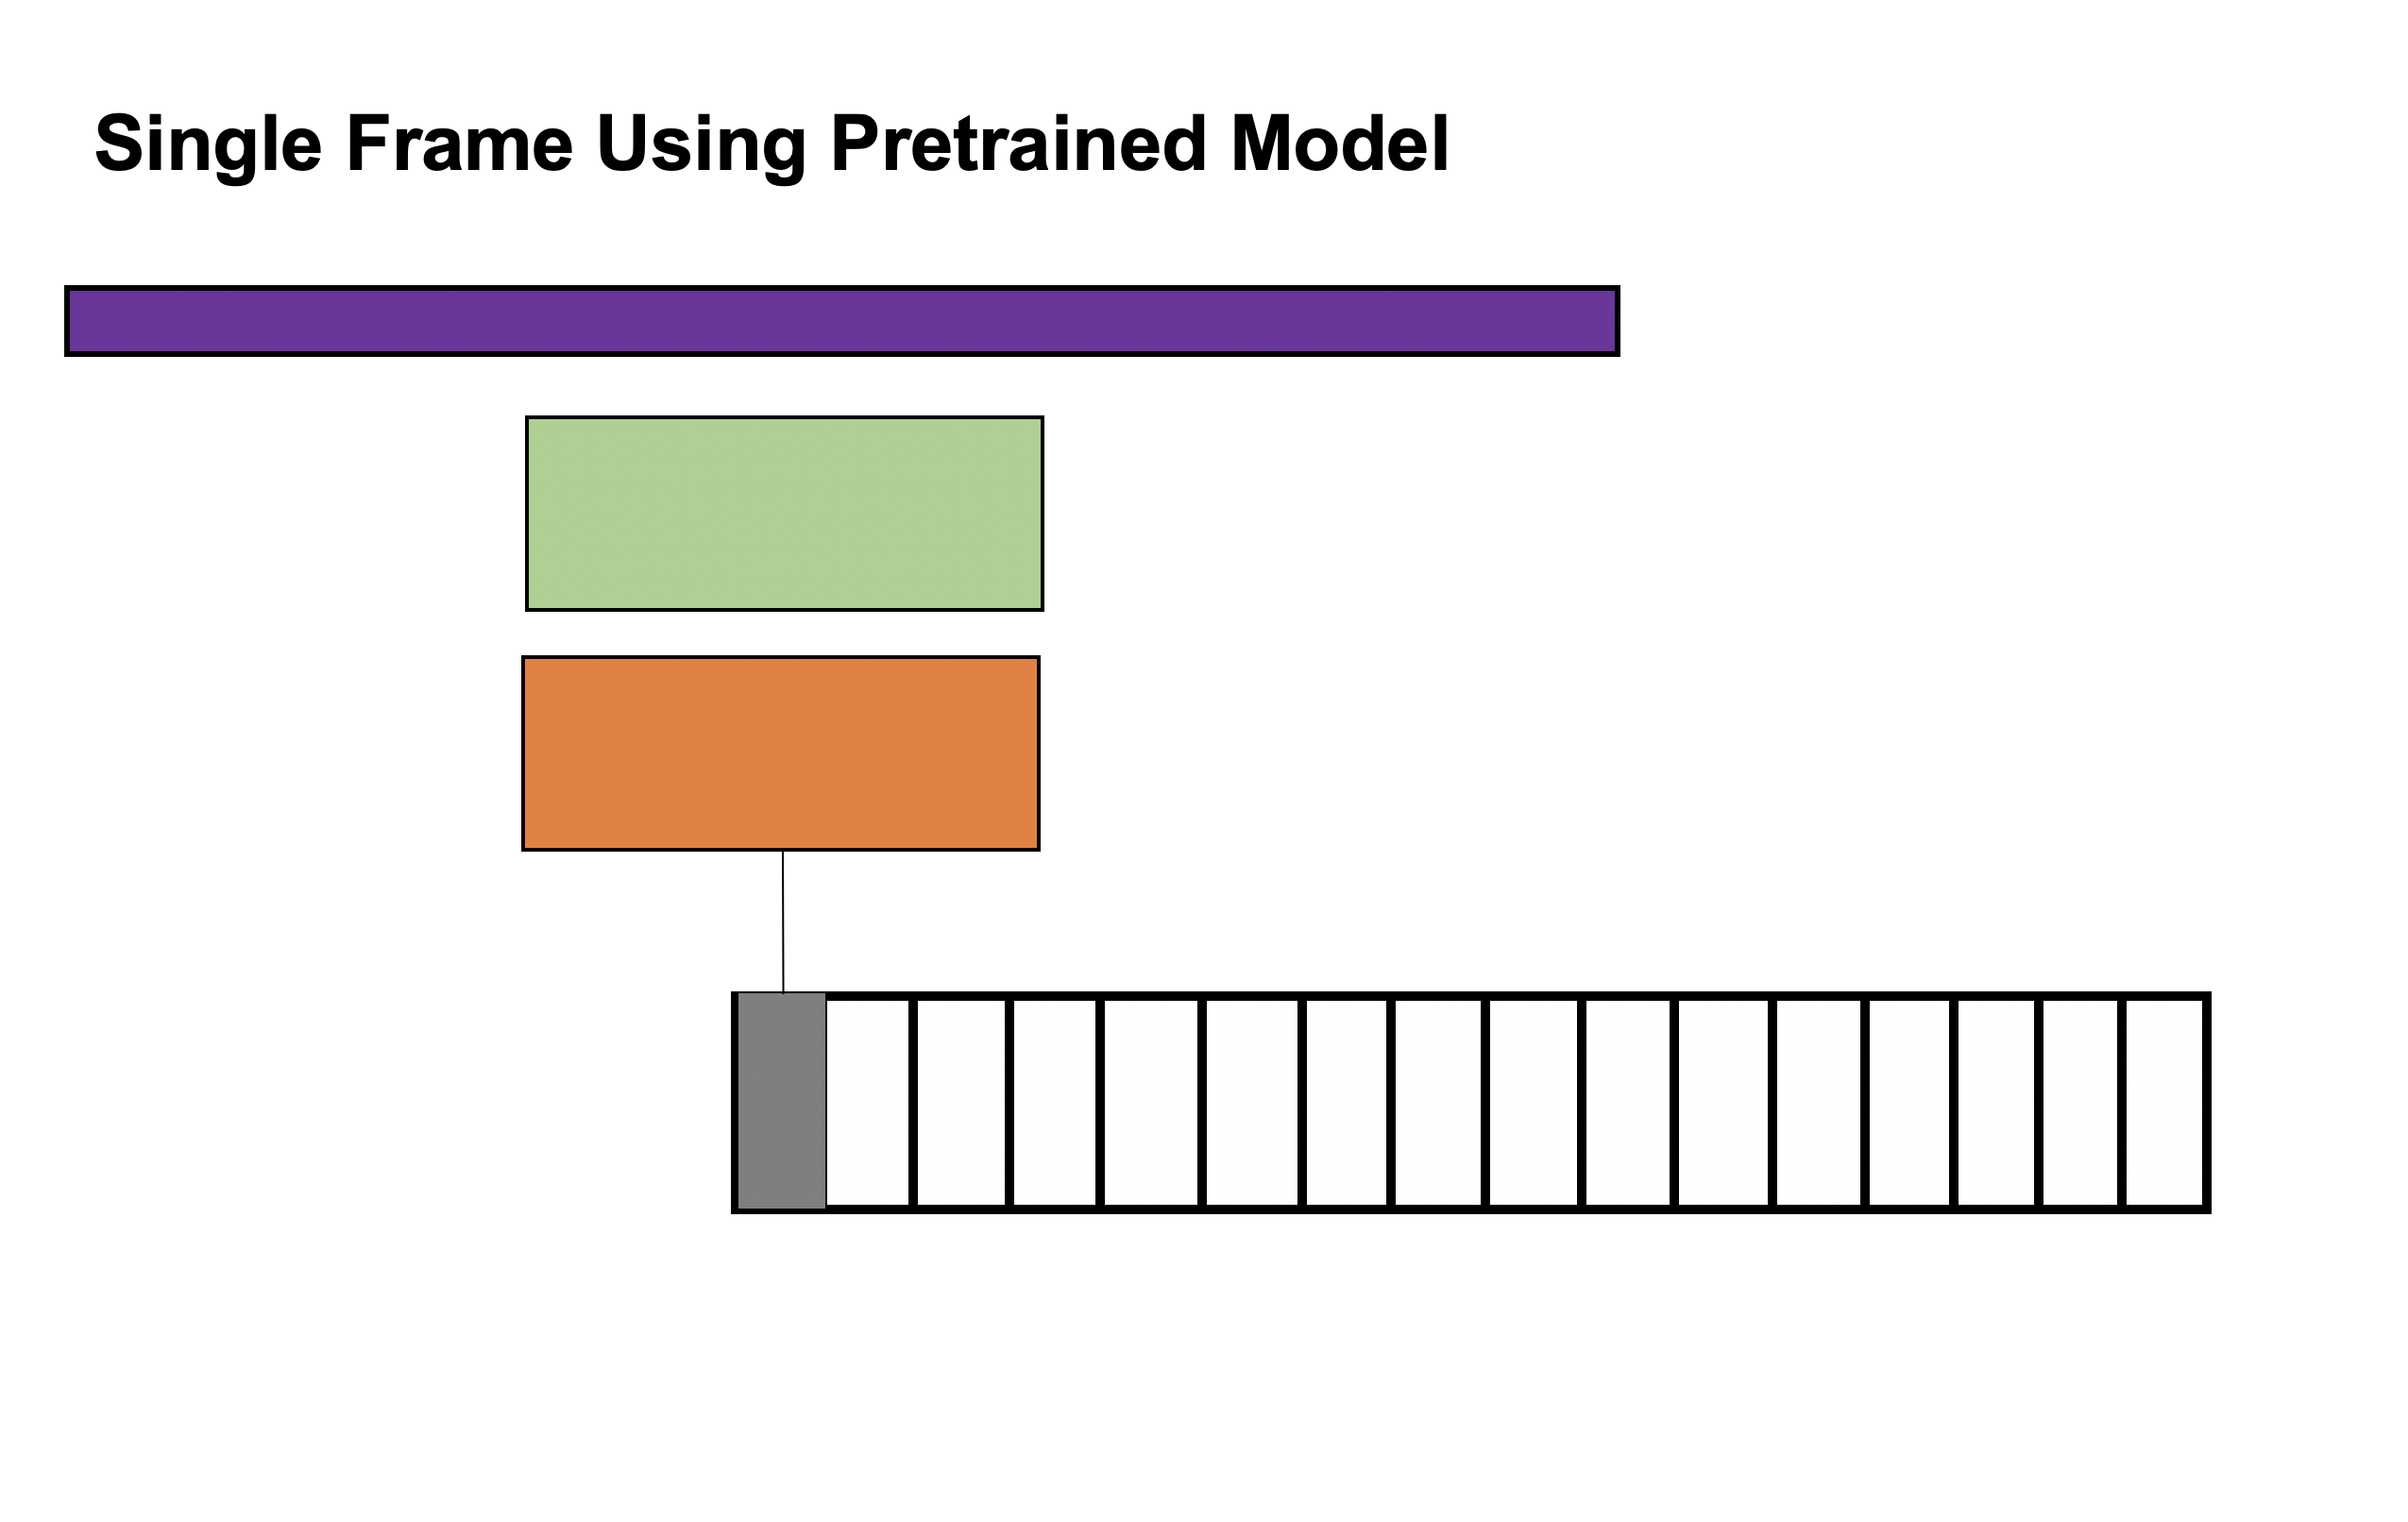
\includegraphics[width=75mm,scale=0.5]{pretrained-single.png}
    \caption{Architectural setup of the pre-trained models, the frame is feed to the pre-trained model layer which has a  50\% dropout applied to it, followed by a global average pooling layer and then the output layer. 
}
    \label{fig:pretrained-single}
\end{figure}


\section{Performance of pre-trained models with multi frames}
This experiment looks to add some temporal information to using the pre-trained models discussed previously.  This setup was inspired by the late fusion model in \citep{KarpathyCVPR14} and involved selecting two frames 15 frames apart. Each frame was then passed through a layer with the same pre-trained model using a dropout of 50\%.  This was then combined and passed to the global average pooling layer as seen in figure \ref{fig:pretrained-late}. This experiment was done for the VGG19, mobileNetv2, inception, ResNet. 
The models were trained similar to the previous experiment using stochastic gradient descent with a learning rate of 0.1, momentum of 0.9,  decay of 0.0005 . These models also ran on the UCL cluster using 128GB of RAM and 2 GPUs.

\begin{figure}
\centering
    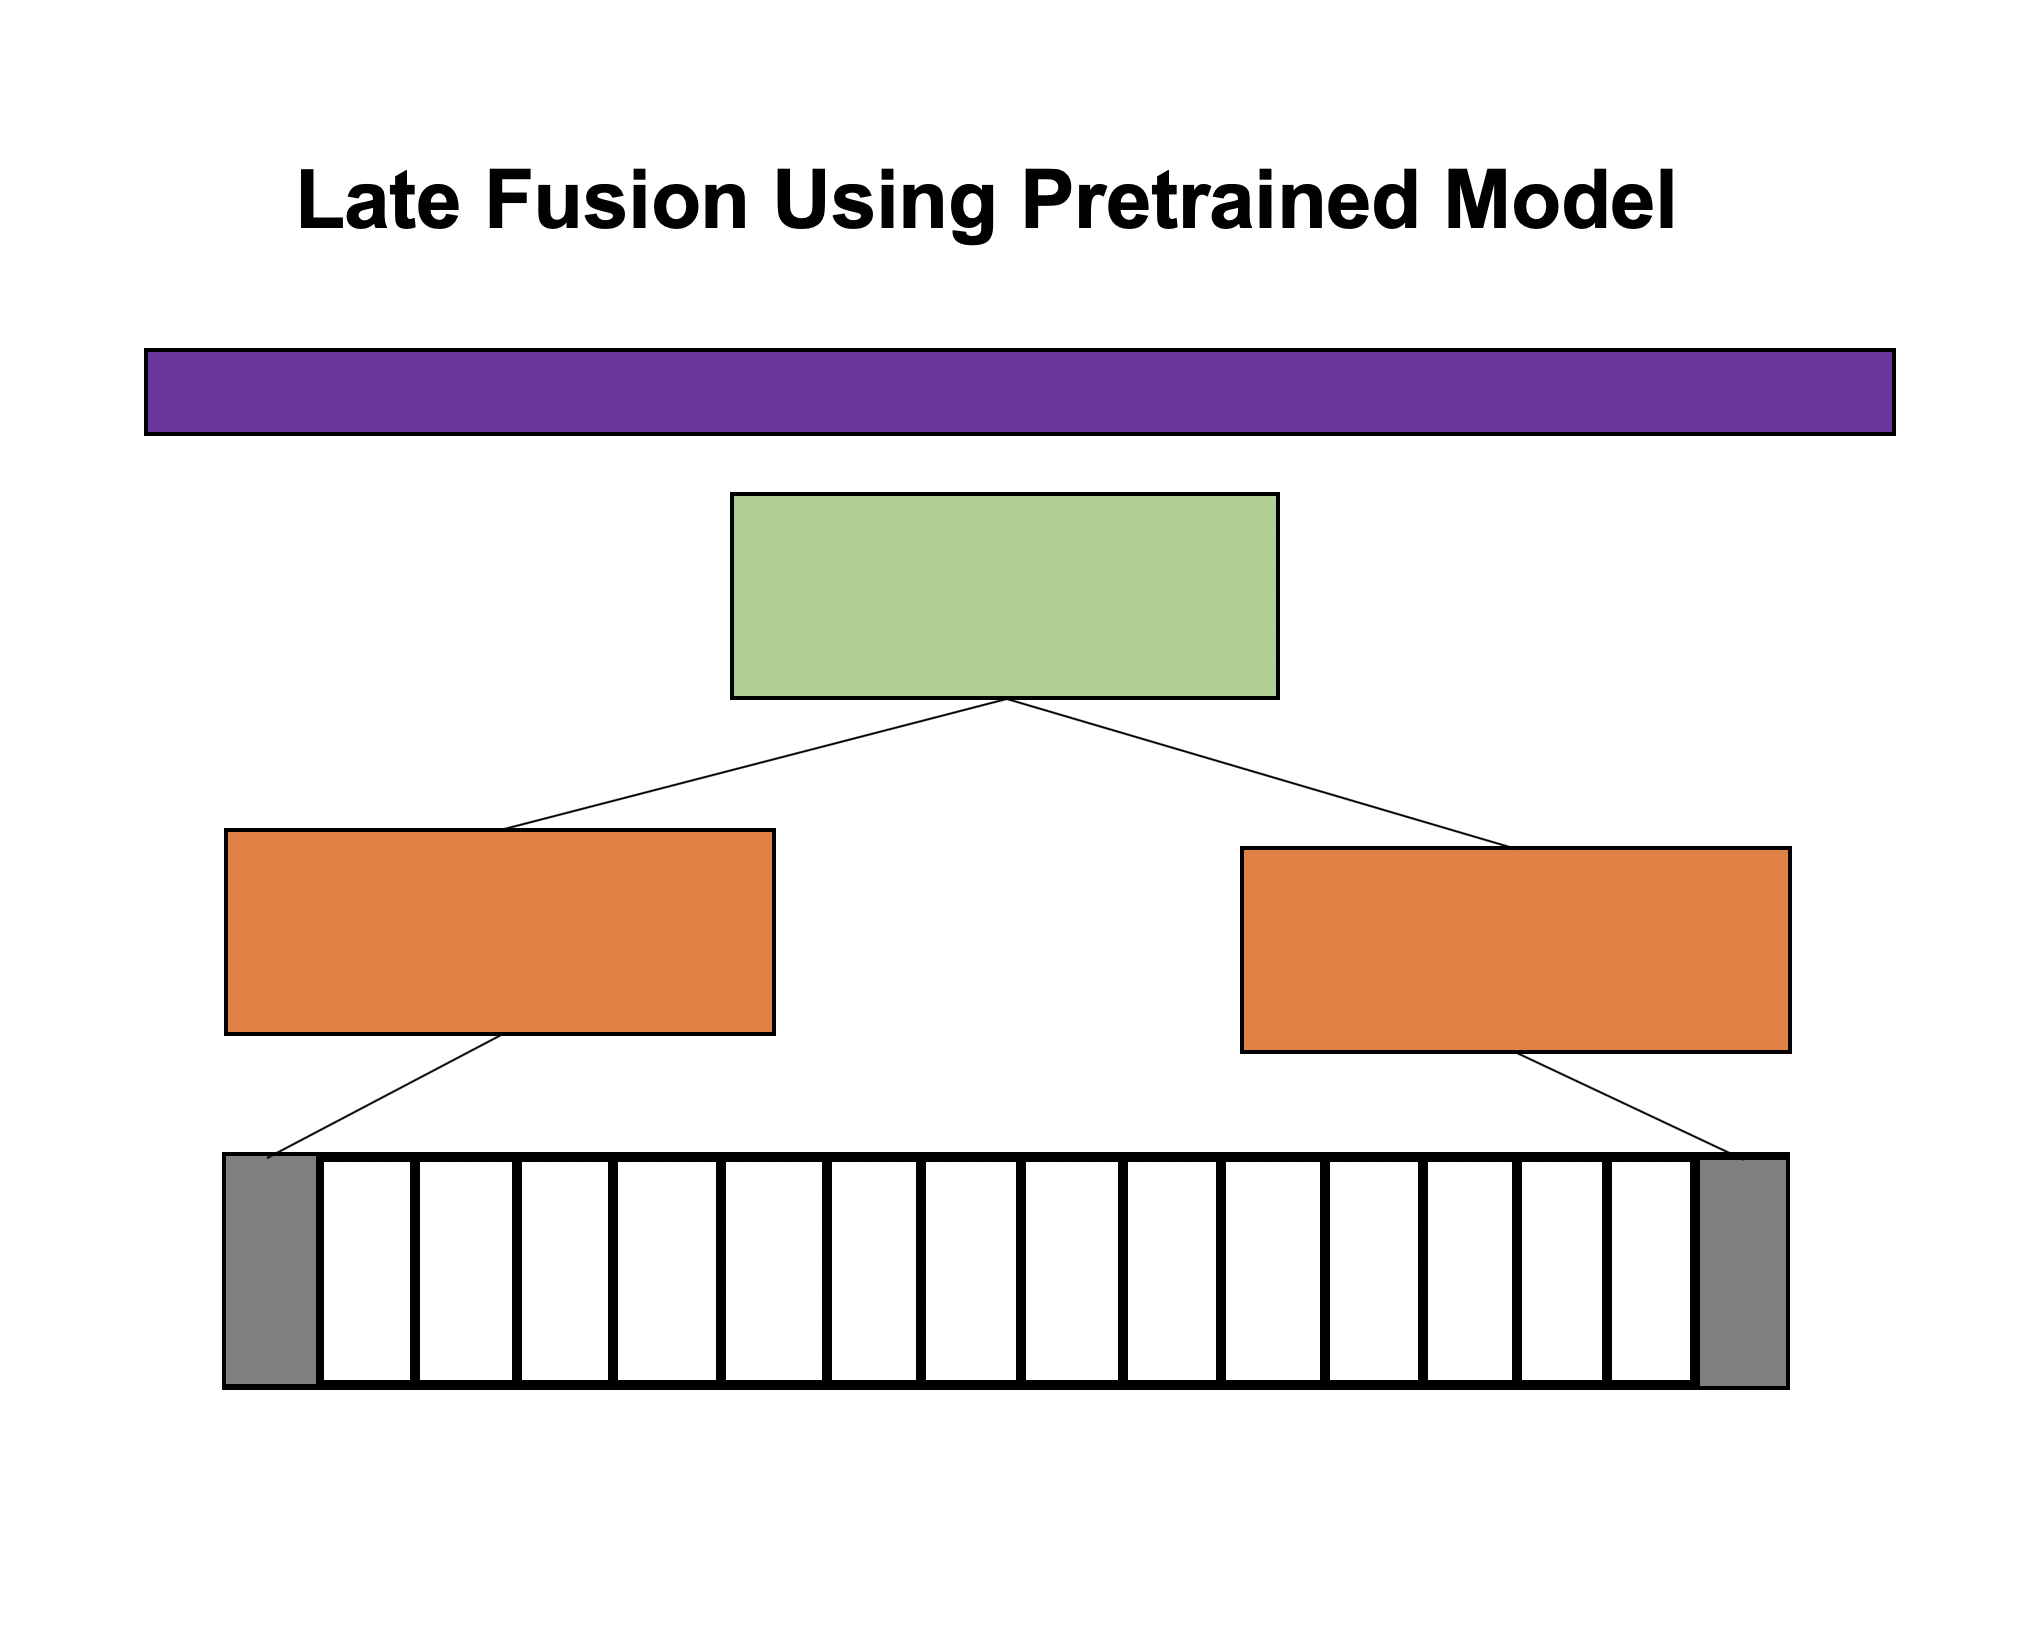
\includegraphics[width=75mm,scale=0.5]{pretrained-late.png}
    \caption{Structure of pre trained late fusion models}
    \label{fig:pretrained-late}
\end{figure}


\section{Data Augmentation}
%t need to find papers for the 255 thing%
\citep{KarpathyCVPR14} paper talks about using certain augmentation on data. The augmentation, as discussed in the setup chapter of this report, were attempted using tensorflow libraries image library on the training dataset. The preprocessed were then applied to the training data for a single frame model using batch normalization and stochastic gradient descent with a momentum of 0.9,  decay of 0.0005 and a learning rate of $1e^{-3}$.  This model was then validated again the test set. And was ran on the UCL cluster using 128GB of RAM and 2 GPUs.




%\section{Data Augmentation}
%To improve traing time different cluster configures where used with different ram sized cpu vs gpu and parallel machines%



% \subsection{RNN}
% trying


    \chapter{Results}
  \section{LRN vs Batch normalization}
The table \ref{lrnvsbatch} shows the training performance of the models using both batch normalization and local response normalization. From the table below it is clear to see batch normalization is superior normalization. This is as expected because as  dicussed in \citep{ioffe2015batch}  batch normalization tends to achieves the same accuracy with 14 times fewer training steps. There is also the possibility that the local response normalization did not work well because of issues with the implementation or the wrong parameters use for training such as an inefficient learning rate. There  epoch levels for the more complex models like the slow fusion and late fusion were less because they took about 3 plus hours to train per epooch hence the were not able to complet under the clock time. 
\begin{table}[h!]
\centering
\begin{tabular}{ |l|c|c|c| } 
 \hline
 Model & Epoch & Accuracy & Loss \\ 
  \hline
 Single frame LRN & 10 & 0.0479 & 4.2867 \\ 
 Single frame batch  & 10 & 0.9158 & 0.3518 \\ 
 Early fusion LRN & 10 & 0.0893 & 3.9725 \\
 Sarly fusion batch & 10 & 0.9467 &  0.2447  \\
 Late fusion LRN & 3 & 0.0194 &  4.6014  \\
 Late fusion batch & 3 & 0.3929  & 2.5302 \\
 Slow fusion LRN & 3 & 0.0246 & 4.5663  \\
 Slow fusion batch & 3 & 0.3764  & 2.5714  \\
 \hline
\end{tabular}
\caption{Batch vs LRN normalization}
\label{lrnvsbatch}
\end{table}

\section{Temporal relationships}
Table \ref{fusions} compares the performance of the single frame, early fusion, late fusion and slow fusion models against the test dataset. Originally all models were planned to run for the same for about 20 epochs using the same early stopping at a 99\% accuracy, but because of the long-running time of the slow and late fusion models all models they were ran for 10 epochs. The performance of the slow fusion model on the training data at 10 epoch was a loss of 0.6477 and then an accuracy of 0.8765.  For the late fusion model, it had a loss of 0.2779  and an accuracy 0.9477.  The early fusion and single frame fusion model  both stopped at 16 epochs because of the early stopping setup. The early fusion had a loss of 0.0179  and an accuracy 0.9995 after 16 epochs while the single frame model had a loss of 0.0186 and an accuracy 0.9994.
From table Table \ref{fusions} we can see that all the models clearly overfitted with the early fusion model performing best then the sing frame model.  Which is not at all similar to the models in \citep{KarpathyCVPR14}, were the flow fusion on average performed better followed by the single-frame fusion model then the late fusion model the finally, the early fusion model. The models as described in \citep{KarpathyCVPR14}, generally did better than the models in the experiment; this could be because of wrong implementation and inefficient hyperparameters and optimization methods.  The overfitting compared to the \citep{KarpathyCVPR14} could also be because of the large amount of augmented varied data used for training in \citep{KarpathyCVPR14}  vs the small non augmented dataset used in this project.
 
\begin{table}[h!]
\centering
\begin{tabular}{ |l|c|c|c| } 
 \hline
 Model & Epoch & Accuracy & Loss \\ 
  \hline
 Single frame batch  & 16   & 0.2360 & 6.3380 \\ 
 Early fusion batch  & 16 & 0.2437 &  6.4750 \\
 Late fusion batch   & 10 & 0.2115 & 5.5500 \\
Slow fusion batch   & 10 & 0.1961& 5.8697\\
 \hline
\end{tabular}
\caption{ Performance of single frame, early fusion, late fusion and slow fusions models against the test dataset}
\label{fusions}
\end{table}

\section{Optimization}
%todo mention next step is parameter searching using different techniques
There was not much improvement in the loss using other optimization method as seen in table \ref{optim}.  This would be most likely due to inefficient hyperparameters used for both the Adam and the RMS prop optimization methods. The RMS prop optimization was cut short due to some issues during running but bad performace can be seeen even at 7 epochs.
\begin{table}[h!]
\centering
\begin{tabular}{ |c|c|c|c|c|c| } 
 \hline
  \multicolumn{2}{|c|}{ } &
 \multicolumn{2}{|c|}{Training } &
 \multicolumn{2}{|c|}{validation} \\
 \hline
 model & epoch & accuracy & loss & accuracy & loss \\ 
  \hline
 SGD & 10 &  0.9546 & 0.2101  & 0.2233 &5.4826 \\ 
 Adam & 10 &0.0111 & 15.9395 & 0.01084 &15.9446 \\
 RMS-prop & 7 & 0.0073 & 15.9985 & - & -  \\ 
 \hline
\end{tabular}
\caption{Results of single frame model performance using sgd with momentum, adam and RMS-prop optimization methods}
\label{optim}
\end{table}


\section{Random Single Frame}
The table \ref{randomSingleFrame} shows the performance of the single frame model which randomly selects a frame from the first 25 frames for each training example. This model did exceeding well that all other models based off the models in \citep{KarpathyCVPR14}.  The training data has an accuracy of 70\%, and the test data had an accuracy of about 54\%. There is still a bit of overfitting however, not compared to the single frame model. The single frame model was also trained using the 7th frame from the videos as this was another assumption of where the frames were taken from based on the images from \citep{KarpathyCVPR14}. The 7th frame single frame model also did not do nearly as well of the test set. There is still alot to be investigated here as it proposes that rather than looking at temporal features it might be better to have a diverse set of images for each action for training.  The bad performances of the single-frame model at the first frame and the 7th frame could also be due to a need for an earlier stopping as the random single frame model trained to about 70\% accuracy. 

\begin{table}[h!]
\centering
\begin{tabular}{ |c|c|c|c|c|c| } 
 \hline
  \multicolumn{2}{|c|}{ } &
 \multicolumn{2}{|c|}{Training } &
 \multicolumn{2}{|c|}{validation} \\
 \hline
 model & epoch & accuracy & loss & accuracy & loss \\ 
  \hline
   Random  single frame model& 20 &  0.7033 & 1.0837 & 0.5388 &1.7621\\ 
Single frame model @ 1  & 10 &   0.9546 & 0.2101 & 0.2234 & 5.4826\\ 
Single frame model @ 7  & 10 &   0.9455 & 0.2345 & 0.2086 &5.3418\\ 
 \hline
\end{tabular}
\caption{Performance of the randon single frame model against a single frame model using the first frame (@1) and the 7th frame(@7)}
\label{randomSingleFrame}
\end{table}


\section{ Performance of pre-trained models}
Table \ref{pretrained} below shows the results from using the pre-trained models; Inception, VGG19, MobileNetv2 and ResNet. The models all ran for 3 epoch, and all had about the same accuracy, which was about 1\% for both the training and test data.  This could because more regularization was needed for these more complex models. For better performance, the models would also have needed to run for a longer time, probably with a higher learning rate or a better optimization method to improve the loss after each epoch.  It was also discovered that the models where accidentally ran with an RMS prop optimization and a learning rate of  0.1 with $\rho$ set to 0.9, and the decay set to 0.0. These parameters must have been extremely inefficient, leading to the bad performance. 

\begin{table}[h!]
\centering
\begin{tabular}{ |c|c|c|c|c|c| } 
 \hline
  \multicolumn{2}{|c|}{ } &
 \multicolumn{2}{|c|}{Training } &
 \multicolumn{2}{|c|}{validation} \\
 \hline
 model & epoch & accuracy & loss & accuracy & loss \\ 
  \hline
     Inception & 3 & 0.0106 & 748.3878 & 0.0116&749.3610 \\ 
 MobileNetv2 & 3 &0.0106 &  745.1055  & 0.0116&749.3610\\
  ResNet & 3 & 0.0106 & 746.8202 & 0.0116 &749.3610  \\ 
  VGG19 & 3 &  0.0106 & 745.9383 & 0.0116 &749.3610\\
 
 \hline
\end{tabular}
\caption{Performace of models using pretrained models ; Inception,VGG19, MobileNetv2 and ResNet}
\label{pretrained}
\end{table}

\section{ Performance of pre-trained models with multi frames}
As seen in table \ref{pretrainedlate}, the late fusion models using the pre-trained models; Inception, VGG19,  MobileNetv2 and ResNet performed much better than their equivalents single frame models. This better performance could be a mix of more information from the additional frame or the fact that the sgd optimization used for all the models with a momentum of 0.9, a decay of 0.0005 and a learning rate of 0.1, was a better optimization method for training.  All models also overfitted with some worse than others.  This could breed the argument that maybe some architectures are more vulnerable to overfitting than others. 

\begin{table}[h!]
\centering
\begin{tabular}{ |c|c|c|c|c|c| } 
 \hline
  \multicolumn{2}{|c|}{ } &
 \multicolumn{2}{|c|}{Training } &
 \multicolumn{2}{|c|}{validation} \\
 \hline
 model & epoch & accuracy & loss & accuracy & loss \\ 
  \hline
   Inception & 3 & 0.6900 & 2.9084 & 0.2297 &33.1893 \\ 
    MobileNetv2 & 3 & 0.8830  & 1.1337 & 0.2361 & 19.5433\\
  ResNet & 3 & 0.9298  & 0.7305 & 0.0095 & 24.4215   \\ 
 VGG19 & 3 & 0.3210 & 3.6636 & 0.0098 & 16.9945 \\
 \hline
\end{tabular}
\caption{Performance of late models using pretrained models ; Inception,VGG19, MobileNetv2 and ResNet}
\label{pretrainedlate}
\end{table}

\section{ Data Augmentation}
As seen in table \ref{dataAug}, the data augmentation did not make much of a difference to the performance of the single frame model. In fact, the results in a worse performance probability due to the loss of information in the images from the resizing and cropping.  This is not to say data augmentation is not beneficial, but rather more forms need to be explored for this dataset and task. 

\begin{table}[h!]
\centering
\begin{tabular}{ |c|c|c|c|c|c| } 
 \hline
  \multicolumn{2}{|c|}{ } &
 \multicolumn{2}{|c|}{Training } &
 \multicolumn{2}{|c|}{validation} \\
 \hline
 model & epoch & accuracy & loss & accuracy & loss \\ 
  \hline
   Inception & 20 & 0.6972 & 1.1184 & 0.1065 &6.0586 \\ 
 \hline
\end{tabular}
\caption{Pretrained models 1 epooch results}
\label{dataAug}
\end{table}

\section{ Computation}
On the UCL clusters, the use of different computing resources was explored, such as the used of RAM and the use of GPU vers CPU. Overall, for most models, the speed per each epoch increased significantly when going from 8GB to 128GB of RAM and when using a GPU versus without. 
 
\chapter{Conclusions}
\label{conclusion}

From implementing various models, TensorFlow and Keras API truly provide a user-friendly and efficient way of implementing these models through the already built-in functions and methods such as the Keras layers and models building tools functionality.  Other benefits of these frameworks is how easily customized methods functionality can be added, how it allows for easy used of pre-trained models and how effortless the frameworks work together. 
 
In terms of the performance of the constructed models from \citep{KarpathyCVPR14}, it is clear to see that there can be difficulties in reproducing model performance, especially when using a different dataset. As this will require a different set of optimization methods and hyperparameters.  Also, in order to get great performances from pre-trained models;  a vast amount of fine tuning of the hyperparameters and regularization techniques are required.

Exploring these hyperparameters will be the next step to the project. This will involve exploring what tools,  can be used with TensorFlow and Keras to explore hyperparameters more systematically and efficiently. Overall, in terms of model design, an orthogonal approach should have been taken, looking at architecture performance then optimization fully. 

As for the used of temporal features, nothing conclusive was decided as all models required better optimization and regularization to help with overfitting. However, a possible theory is that a single frame model is just as efficient as other models considering temporal features. Moreover, it can be even more efficient if trained with frames at different points in time from different videos. Another next step from this project will be to also look into Recurrent neural networks which are designed to look at sequence data which are inclusive of videos. 
% \addcontentsline{toc}{chapter}{Appendices}

% The \appendix command resets the chapter counter, and changes the chapter numbering scheme to capital letters.
%\chapter{Appendices}
\appendix
\chapter{An Appendix About Stuff}
\label{appendixlabel1}
(stuff)

% \chapter{Another Appendix About Things}
% \label{appendixlabel2}
% (things)

% \chapter{Colophon}
% \label{appendixlabel3}
% \textit{This is a description of the tools you used to make your thesis. It helps people make future documents, reminds you, and looks good.}

% \textit{(example)} This document was set in the Times Roman typeface using \LaTeX\ and Bib\TeX , composed with a text editor. 
 % description of document, e.g. type faces, TeX used, TeXmaker, packages and things used for figures. Like a computational details section.
% e.g. http://tex.stackexchange.com/questions/63468/what-is-best-way-to-mention-that-a-document-has-been-typeset-with-tex#63503

% Side note:
%http://tex.stackexchange.com/questions/1319/showcase-of-beautiful-typography-done-in-tex-friends 
% You could separate these out into different files if you have
%  particularly large appendices.

% This line manually adds the Bibliography to the table of contents.
% The fact that \include is the last thing before this ensures that it
% is on a clear page, and adding it like this means that it doesn't
% get a chapter or appendix number.
\addcontentsline{toc}{chapter}{Bibliography}

% Actually generates your bibliography.
\bibliography{References}

% All done. \o/
\end{document}
